% This is the Reed College LaTeX thesis template. Most of the work
% for the document class was done by Sam Noble (SN), as well as this
% template. Later comments etc. by Ben Salzberg (BTS). Additional
% restructuring and APA support by Jess Youngberg (JY).
% Your comments and suggestions are more than welcome; please email
% them to cus@reed.edu
%
% See http://web.reed.edu/cis/help/latex.html for help. There are a
% great bunch of help pages there, with notes on
% getting started, bibtex, etc. Go there and read it if you're not
% already familiar with LaTeX.
%
% Any line that starts with a percent symbol is a comment.
% They won't show up in the document, and are useful for notes
% to yourself and explaining commands.
% Commenting also removes a line from the document;
% very handy for troubleshooting problems. -BTS

% As far as I know, this follows the requirements laid out in
% the 2002-2003 Senior Handbook. Ask a librarian to check the
% document before binding. -SN

%%
%% Preamble
%%
% \documentclass{<something>} must begin each LaTeX document
\documentclass[12pt,twoside]{reedthesis}
% Packages are extensions to the basic LaTeX functions. Whatever you
% want to typeset, there is probably a package out there for it.
% Chemistry (chemtex), screenplays, you name it.
% Check out CTAN to see: http://www.ctan.org/
%%
\usepackage{graphicx,latexsym}
\usepackage{amsmath}
\usepackage{amssymb,amsthm}
\usepackage{longtable,booktabs,setspace}
\usepackage{chemarr} %% Useful for one reaction arrow, useless if you're not a chem major
\usepackage[hyphens]{url}
% Added by CII
\usepackage{hyperref}
\usepackage{lmodern}
\usepackage{float}
\floatplacement{figure}{H}
% End of CII addition
\usepackage{rotating}

% Next line commented out by CII
%%% \usepackage{natbib}
% Comment out the natbib line above and uncomment the following two lines to use the new
% biblatex-chicago style, for Chicago A. Also make some changes at the end where the
% bibliography is included.
%\usepackage{biblatex-chicago}
%\bibliography{thesis}


% Added by CII (Thanks, Hadley!)
% Use ref for internal links
\renewcommand{\hyperref}[2][???]{\autoref{#1}}
\def\chapterautorefname{Chapter}
\def\sectionautorefname{Section}
\def\subsectionautorefname{Subsection}
% End of CII addition

% Added by CII
\usepackage{caption}
\captionsetup{width=5in}
% End of CII addition

% \usepackage{times} % other fonts are available like times, bookman, charter, palatino

% Syntax highlighting #22

% To pass between YAML and LaTeX the dollar signs are added by CII
\title{Added Variable Plot Importance and Joint Added Variable Plot Importance
Measures for Random Forests}
\author{Emerson H. Webb}
% The month and year that you submit your FINAL draft TO THE LIBRARY (May or December)
\date{May 2018}
\division{Mathematics and Natural Sciences}
\advisor{Andrew Bray}
\institution{Reed College}
\degree{Bachelor of Arts}
%If you have two advisors for some reason, you can use the following
% Uncommented out by CII
% End of CII addition

%%% Remember to use the correct department!
\department{Mathematics}
% if you're writing a thesis in an interdisciplinary major,
% uncomment the line below and change the text as appropriate.
% check the Senior Handbook if unsure.
%\thedivisionof{The Established Interdisciplinary Committee for}
% if you want the approval page to say "Approved for the Committee",
% uncomment the next line
%\approvedforthe{Committee}

% Added by CII
%%% Copied from knitr
%% maxwidth is the original width if it's less than linewidth
%% otherwise use linewidth (to make sure the graphics do not exceed the margin)
\makeatletter
\def\maxwidth{ %
  \ifdim\Gin@nat@width>\linewidth
    \linewidth
  \else
    \Gin@nat@width
  \fi
}
\makeatother

\renewcommand{\contentsname}{Table of Contents}
% End of CII addition

\setlength{\parskip}{0pt}

% Added by CII

\providecommand{\tightlist}{%
  \setlength{\itemsep}{0pt}\setlength{\parskip}{0pt}}

\Acknowledgements{
I want to thank a few people.
}

\Dedication{
You can have a dedication here if you wish.
}

\Preface{

}

\Abstract{
The preface pretty much says it all. \par

Second paragraph of abstract starts here.
}

	\usepackage{tikz, algorithm}
	\usepackage[noend]{algpseudocode}
% End of CII addition
%%
%% End Preamble
%%
%

\usepackage{amsthm}
\newtheorem{theorem}{Theorem}[chapter]
\newtheorem{lemma}{Lemma}[chapter]
\theoremstyle{definition}
\newtheorem{definition}{Definition}[chapter]
\newtheorem{corollary}{Corollary}[chapter]
\newtheorem{proposition}{Proposition}[chapter]
\theoremstyle{definition}
\newtheorem{example}{Example}[chapter]
\theoremstyle{definition}
\newtheorem{exercise}{Exercise}[chapter]
\theoremstyle{remark}
\newtheorem*{remark}{Remark}
\newtheorem*{solution}{Solution}
\begin{document}

% Everything below added by CII
  \maketitle

\frontmatter % this stuff will be roman-numbered
\pagestyle{empty} % this removes page numbers from the frontmatter
  \begin{acknowledgements}
    I want to thank a few people.
  \end{acknowledgements}

  \hypersetup{linkcolor=black}
  \setcounter{tocdepth}{2}
  \tableofcontents

  \listoftables

  \listoffigures
  \begin{abstract}
    The preface pretty much says it all. \par
    
    Second paragraph of abstract starts here.
  \end{abstract}
  \begin{dedication}
    You can have a dedication here if you wish.
  \end{dedication}
\mainmatter % here the regular arabic numbering starts
\pagestyle{fancyplain} % turns page numbering back on

\chapter*{Introduction}\label{introduction}
\addcontentsline{toc}{chapter}{Introduction}

This thesis is about utilizing the predictive capabilities of random
forests for statistical inference via variable importance measures. The
random forest is a statistical learning algorithm developed by Leo
Breiman and his collaborators in the early 2000's that leverages bagging
and CART (Classification and Regression Trees) methodology to produce
quite good predictions of an underlying classification or regression
surface. Random forests often outperform classical linear models, are
simple to set-up and train, and come with few assumptions about the
underlying data generating process. For this thesis, we are interested
in the use of random forest variable importance measures for statistical
inference. More specifically, random forest variable importance measures
are often unstable with respect to correlated predictors, so our focus
is on developing variable importance measures that can produce stable
results even when there are correlated predictors in the dataset. \par

Machine learning approaches to regression can often produce models with
good predictive accuracy compared to parametric modelling approaches.
However, machine learning algorithms often lack in the interpretability
and inferential capabilities of more traditional statistical modelling.
The challenge of developing descriptive and inferential tools for
machine learning algorithms is in finding a balance between complexity
and interpretability. While we may want a variable importance measure
that fully utilizes the predictive cabilities of the algorithm, we also
want the variable importance measure to be simple enough for statistical
practitioners to use and interpret. \par

Throughout this thesis we will be primarily interested in the regression
settings for random forests. While random forests are capable of
handling both regression and classification responses, our discussion
will be simpler if we focus just on the regression setting. Also, we
will be assuming that for the data at hand, there exists an underlying
regression function \(Y=f(X)+\varepsilon\) where \(f(X)\) is an
arbitrary, not necessairly linear function, and \(\varepsilon\) is
generally assumed to be Gaussian error, but may have some other error
structure. \par

\chapter{Introduction to Trees, Random Forests, and the
Bootstrap}\label{rmd-basics}

\section{CART}\label{cart}

We begin our discussion of CART (Classification and Regression Trees) by
considering the following problem. Suppose we have data generated from
the piecewise function \(Y=f(X)+\varepsilon\) where {[}at this point
insert a very non-linear piecewise function.{]} with Gaussian error
\(\varepsilon\). One approach to fitting a model to this data would be
to fit a linear regression model. However, the particular form of the
data is not well suited for linear regression due to the non-linearity
of the data. Another approach we might try as follows. We might try to
find a method that can fit a regression line to each piecewise component
of the data. One such method is to fit CART trees. We fit a CART tree to
the data and perform cost-complexity pruning to output the model shown
in figure {[}figure not yet made{]}. In this example, we produced a
regression surface which was able to take into account the piecewise,
non-linear nature of the data and produce a reasonable estimate of the
underlying data generating mechanism. \par

The CART methodology allows us to fit a model that can take into account
non-linear regression or classification surfaces. The basic idea of CART
is that if we can split the predictors into roughly homogenous
partitions in terms of the response \(Y\), then we can fit a simple
model to predict the response of each partition. CART trees were first
introduced by Breiman, Friedman, Olshen, \& Stone (1984) and are a
flexible method, capable of handling classification and regression
settings. \par

More formally, suppose we have a training data set
\(Z=\{Z_1,\ldots,Z_n\}\), where \(Z_i=(X_i,Y_i)\) is an \(p+1\)
dimensional vector in \(\mathbb{R}^{p+1}\). Here we have \(X_i\) is a
\(p\)-dimensional predictor variable and \(Y_i\) is the response. In
particular, we can consider \(Z\) to be a \(n\times (p+1)\) array where
the rows are observations and the columns are the response and predictor
variables. CART works by partitioning the data through binary recursive
splits via optimizing some loss function. Trees in CART are called trees
because partitioning the data through binary recursive splits forms a
tree-like structure. We adopt notation evocative of this tree structure.
Any subset of the training data \(Z\) is called a node while the entire
data set \(Z\) is called the root node. Nodes are of two kinds: they are
either terminal (sometimes called leaves) or not terminal. Non-terminal
nodes are nodes that are split on in the tree growing process, while
terminal nodes are nodes which are not split on. Generally, a node is a
terminal node if some stopping rule is reached. Note that terminal nodes
form a partition of the training data \(Z\). \par

We aim to grow a tree with roughly homogenous terminal nodes in terms of
\(Y\). As Breiman et al. (1984) note, there are several factors that we
need to consider:
\begin{enumerate}
        \item How to select splits of the data.
        
        \item When to stop splitting the data.
        
        \item How to assign classes or values to terminal nodes. 
    \end{enumerate}
CART address point 1 decreasing the nodal impurity of a node \(t\).
Nodal impurity is defined through some nodal impurity measure
\(i(s,t)\), usually the GINI index in the classification setting and the
residual sum of squares in the regression setting. We present the
regression setting and then the classification setting. If we have a
continuous response \(Y\), then we could try to predict \(Y\) by
partitioning the data using the decision tree structure and predicting
that points that fall within a particular partition will take on the
average response on that partition. To choose the best binary split on
the data, we need to search across the splitting variables and splitting
points for the split which maximizes the reduction in the RSS between
the parent node and daughter nodes. In particular, we want to find the
split which maximizes \(RSS_l(j,s)+RSS_r(j,s)\) where \(j\) is the
proposed splitting variable and \(s\) is the proposed splitting point,
and \(RSS_l\) is the RSS of the proposed left node and \(RSS_r\) is the
RSS of the proposed right node. The assignment of response within a node
is given by the average of the response. We present the following
algorithm. \par
\begin{algorithm}
        \caption{Construction of Regression tree}\label{regression tree}
        \begin{algorithmic}[1]
            \While {minimum node size not reached}
                \For {each node $t$ }
                    \For {$j=1,\ldots,p$ and $s=1,\ldots,n$ }
                    \State Compute $RSS_l(j,s)+RSS_r(j,s)$.
                    \EndFor
                    \State Pick the $(j,s)$ which maximizes $RSS_l(j,s)+RSS_r(j,s)$.
                    \State Split the current node into left and right nodes according to $(j,s)$.
                    \State Compute left and right averages, $\text{ave}(y_i|x_i\in t_l)$ and $\text{ave}(y_i|x_i\in t_r)$, respectively. 
                \EndFor
                \State Output the tree $T$.
            \EndWhile
        \end{algorithmic}
    \end{algorithm}
\subsection{Example of Regression
Tree}\label{example-of-regression-tree}

We now provide an example of a regression tree using a simulated data
set we will use throughout this thesis to illustrate important examples.
We made 2000 draws of 3 independent standard normals
\(X_1,X_2,X_3\sim N(0,1)\) and defined the response by the linear
equation \[Y=10X_1-5X_2+\varepsilon,\] where \(\varepsilon\sim N(0,1)\).
Our data set is thus a \(2000\times 4\) array where each row is of the
form \((X_1,X_2,X_3,Y)\). Hence we have two informative predictors
(\(X_1\) and \(X_2\)) and one uninformative predictor (\(X_3\)) in our
simulated data set. For this data set, we ran CART to produce Figure
\ref{tree_ex}. \par  
\begin{figure}
\centering
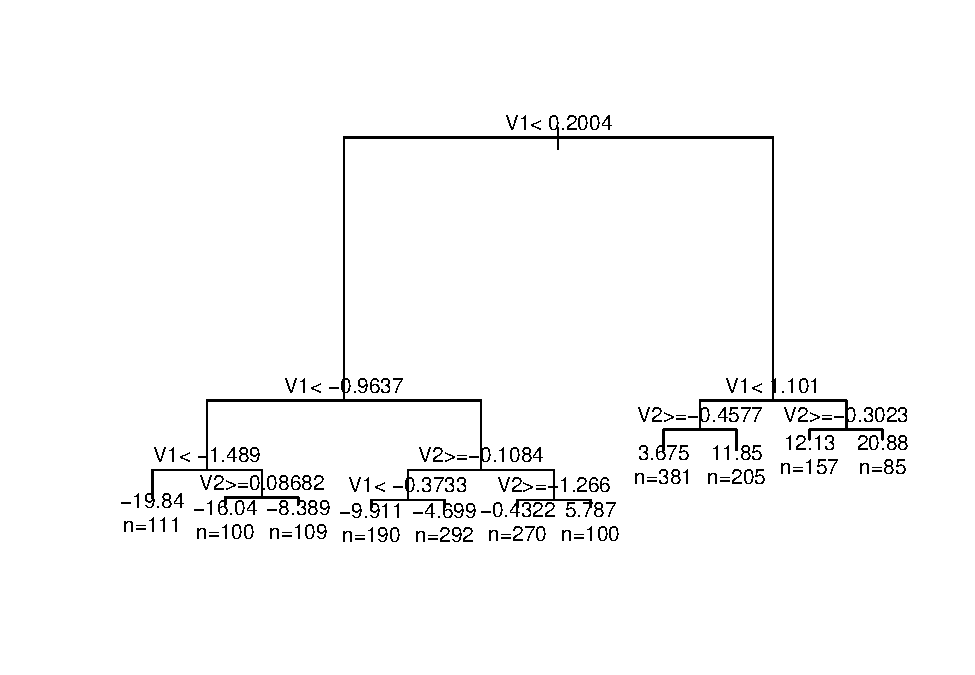
\includegraphics{thesis_files/figure-latex/unnamed-chunk-2-1.pdf}
\caption{\label{fig:unnamed-chunk-2}\label{tree_ex}Example of a Regression
Tree}
\end{figure}
We would like to note that the tree structure produced by CART is quite
easy to interpret. Given some point \(x=(x_1,x_2,x_3)\) in our feature
space, to determine what the prediction for \(x\) should be, we simply
follow the left-right paths down to a terminal node of the tree. We also
note that this regression tree generally reflects the structure of our
data set in the sense that important splits near the base of the tree
tend to be made on \(X_1\), while splits further down in the tree tend
to be on \(X_2\). Furthermore, no splits are made on \(X_3\). In this
scenario, we can visually inspect the tree to determine which predictors
are informative towards predicting the response \(Y\).

\subsection{Classification Trees and Issues with
CART}\label{classification-trees-and-issues-with-cart}

The construction of classification trees is similar to the construction
of regression trees except a different impurity measure must be used.
For the node \(t\) containing \(N_t\) observations, let
\[\hat{p}_{tk}=\frac{1}{N_t}\sum_{x_i\in t} \mathbb{I}(y_i=k)\] where
\(k=0\) or \(k=1\). Then \(\hat{p}_{tk}\) measures the proportion of
observations of class \(k\) in node \(t\). Using the two-class example,
there are several impurity measures available in the classification
setting. The most common measure is perhaps the Gini index defined by
\[2p(1-p).\] Other options include misclassification error
\[1-\max(p,1-p),\] and cross-entropy \[-p\log(p)-(1-p)\log(1-p).\] If
\(t_L\) and \(t_R\) are left and right nodes proposed under the split,
let \(\hat{p}_{tL}\) and \(\hat{p}_{tR}\) be proportion of observations
falling into \(t_L\) and \(t_R\), respectively. Denote the Gini index of
the left node \(t_L\) by \(G_{L}\) and denote the Gini index of the
right node \(t_R\) by \(G_{R}\). Then our splitting criterion is to seek
the spliting variable and splitting point which minimizes
\[\hat{p}_{tL}G_L+\hat{p}_{tR}G_R.\] The case is similar when using
misclassification rate and cross-entropy as the impurity measures. \par

Some issues with CART trees include overfitting and variability. While
there is a stopping criterion for growing the CART trees, often times
naively growing a tree can result in overfitting to the data. One method
of alleviating overfitting is to employ cost-complexity pruning, which
searches for an optimal tree that balances fitting a good predicitve
tree model with overfitting to the data. We do not go into details here,
but point the reader to Hastie, Tibshirani, \& Friedman (2009). \par

A larger issue with trees is their sensitivity to small perturbations in
the data. Allowing the data to vary even a bit can result in a different
tree structure upon refitting. As a statistical learning method, this
means that CART trees are not robust and suffer from high variance, even
when constructed using cost-complexity pruning. To get around this issue
of sensitivity the best solution is to employ bagging and use the random
forest algorithm. \par

\section{Random Forests}\label{random-forests}

Among the limitations of CART discussed in the preceding sections, the
biggest issues ARE perhaps the variability of the method and the issue
of collinearity among predictors. While overfitting can be addressed
using cost-complexity pruning, variability and collinearity are not
fixed by pruning. Random forests deal with these two issues of CART by
introducing a resampling and randomization mechanism. The natural order
is to first discuss bagged forests before turning to random forests.
\par

One method of improving CART trees is to bag them. Bagging, which stand
for bootstrap aggregating, is a variation reduction technique
particularly useful for improving the predictive power of weak learners.
We are interested in bagging CART trees to reduce the variability of
single trees under slight perturbations of the data. Generally bagged
ensembles of learners produce robust predictions in comparison to
running the learner once. \par
\begin{algorithm}
        \caption{Bagged Forest algorithm}\label{bagged forest}
        \begin{algorithmic}[1]
            \For {$b=1,\ldots, B$ }
            \State Draw a bootstrap sample $Z_b^*$ of size $N$ from the training data $Z$.
            \State Grow a CART tree $T_b$ on each bootstrap sample $Z_b^*$.
            \EndFor
            \State Output the bagged forest ensemble $\{T_b\}_{b=1}^B$.
        \end{algorithmic}
    \end{algorithm}
\subsection{How Bagged Forests Work}\label{how-bagged-forests-work}

Bagged forests are an ensemble obtained by taking many bootstrap samples
of the data and fitting a tree to each bootstrapped dataset. In this
case, we grow the trees quite deep and do not employ cost-complexity
pruning. The idea behind this decision is that we want to sufficiently
explore the feature space using a single baggedtree of the forest
ensemble, and since we are also taking an average of the trees, we are
fine with overfitting at least a little bit. As the algorithm above for
bagged forests indicates, the output is an ensemble of trees
\(\{T_b\}_{b=1}^B\). Given a test data point, we form a prediction by
taking the average of predictions given by the tree ensemble:
\[\hat{f}_{bf}^B(x)=\frac{1}{B}\sum_{b=1}^B T_b(x),\] where
\(\hat{f}_{bf}^B\) indicates we are taking the bagged forest estimate of
the underlying regression or classification function using \(B\) many
trees. Note that it is important to be consistent in the choice of
splitting criterion throughout the bagging process. \par

While bagging is a general method, that can be applied, for example, to
methods such as ordinary least squares or general linear models, it has
been shown by Friedman \& Hall (1999) and Chen \& Hall (2003) that
bagging is especially effective when used on highly non-linear models
such as CART trees. Under ideal conditions, bagged estimates of
non-linear estimators reduces both the bias and variance of the
estimator. So bagging trees seem to be effective because of the
reduction to the variance of the estimator, which produces a more robust
prediction. \par

When we bag trees, each observation in the data is not used within each
individual tree. A bootstrap replicate \(Z_b\) of the data \(Z\) will
likely exclude some of the observations within the data. The
observations used within the bootstrap replicate \(Z_b\) is called the
in-bag data while the observations not used within the bootstrap
replicate \(Z_b\) is called the out-of-bag (OOB) data and is denoted by
\(\bar{Z}_b\). The OOB data allows us to approximate the test error of
the ensemble as follows. For simplicity suppose we are in the regression
setting (the classification setting is similar). Then the OOB estimate
of the MSE of the bagged forest is given by
\[MSE_{\textup{OOB}}(T;Z)=\frac{1}{B}\sum_{b=1}^B MSE(T_b;\bar{Z}_b).\]
As the number of trees in the ensemble grows, the OOB estimate of the
MSE for the bagged forest converges to the LOOCV estimate of the MSE for
forest Hastie et al. (2009). \par

A weakness of bagged forests is collinearity between trees Hastie et al.
(2009). This collinearity between trees grown from the bootstrap sample
can be addressed by adding a randomization mechanism in the tree growing
process. When we grow a tree from a bootstrap sample, even with the
randomness induced by resampling from the data, certain features may be
explored at the expense of other just as interesting features. This is a
particular issue with collinear predictors. If two predictors are
collinear, then the bagged forest might consistently choose one
predictor over another even if the predictor not chosen leads to splits
that are just as informative. This is due in part to the greedy nature
of the CART algorithm when searching for optimal splits over the feature
space. The algorithm does not take into account the second best or third
best splits. Furthermore, it is not difficult to see that bagging will
generally produce an ensemble of trees that are quite similar to one
another, subject to some perturbations. These trees will be strongly
correlated with other trees in the ensemble, so if there is a less
explored part of the feature space, then the ensemble will struggle to
produce good predictions over that region. \par

\subsection{The Random Forest
Algorithm}\label{the-random-forest-algorithm}

Random Forests deal with this issue of correlated trees and collinearity
among predictors by choosing at random only \(m\leq p\) of the
predictors to be considered as candidate splitting variables at each
split in each tree in the ensemble. This randomness further reduces the
variance of the bagged forest by decorrelating the trees in the
ensemble. Furthermore, while individually the trees may perform worse
than a single pruned tree, collectively the ensemble has a better chance
of exploring the feature space fully. \par
\begin{algorithm}
        \caption{Random Forest algorithm}\label{random forest}
        \begin{algorithmic}[1]
            \For {$b=1,\ldots, B$ }
            \State Draw a bootstrap sample $Z_b^*$ of size $N$ from the training data $Z$.
            \State Grow the CART tree $T_b$ on $Z_b^*$ with the following modification:
            \While {minimum node size $n_{\min}$ not reached across $T_b$} 
            \State Select $m\leq p$ candidate splitting variables at random.
            \State Pick the best splitting variable and splitting point among the $m$ variables selected at random.
            \State Split the node into two daughter nodes.
            \EndWhile
            \EndFor
            \State Output the random forest ensemble $\{T_b\}_{b=1}^B$.
        \end{algorithmic}
    \end{algorithm}
To form a prediction at a test point \(x\), we have in the regression
setting \[\hat{f}_{rf}^B(x)=\frac{1}{B}\sum_{b=1}^B T_b(x).\] \par

\subsection{Variable Importance
Measures}\label{variable-importance-measures}

One of the outputs of random forests is the variable importance (VI)
measure. There are two main variable importance measures in common use,
with the choice of VI measure varying depending on the setting and
splitting criterion chosen. The first choice is the Mean Decrease in
Impurity (MDI) which is typically used in the classification setting
where the GINI index or Shannon entropy is used as the splitting
criterion. The second choice is Mean Decrease in Accuracy (MDA) which is
typically used in the regression setting where RSS has been used as the
splitting criterion. The idea of MDI is to find how much the nodal
impurity \(p(t)\Delta i(s,t)\) decreases for all nodes \(t\) in which
the variable of interest \(X_j\) is used and to take that average over
all trees in the ensemble. Note that \(p(t)\) is the proportion of
observations of a particular class in the node \(t\) and
\(\Delta i(s,t)\) is the decrease in impurity over the node \(t\) when
variable \(X_j\) is chosen. More important variables are those which are
on average more often chose for splits and which also contribute most to
reducing the nodal impurity of the trees. \par
\begin{algorithm}
        \caption{MDI Variable Importance}\label{mdi variable importance}
        \begin{algorithmic}[1]
            \State Grow a random forest $\{T_b\}_{b=1}^B$.
            \For {$j=1,\ldots,p$ }
                \For {$b=1,\ldots,B$ }
                \State Compute the importance of $X_j$ in $T_b$ as $VI_b(X_j)=\sum_{t\in T_b} \mathbb{I}(j_t=j)p(t)\Delta i(s,t)$ to be the sum of the decrease in impurity over nodes where variable $X_j$ is used .
                \EndFor
                \State Compute the importance of $X_j$ in the random forest to be $VI(X_j)=\frac{1}{B}\sum_{b=1}^B VI_b(X_j).$
            \EndFor
        \end{algorithmic}
    \end{algorithm}
The idea of MDA is to measure for each variable \(X_j\), on average how
much the predictive accuracy of the forest as measured using RSS suffers
when the \(X_j\) component is permuted across observations within the
OOB dataset \(\bar{Z}_b\) of each tree \(T_b\) in the ensemble. \par
\begin{algorithm}
        \caption{MDA Variable Importance}\label{mda variable importance}
        \begin{algorithmic}[1]
            \State Grow a random forest $\{T_b\}_{b=1}^B$.
            \For {$j=1,\ldots,p$ }
            \For {$b=1,\ldots,B$ }
            \State Permute the $X_j$ component of $Z_b$ to obtain the dataset $Z_b^j$, where $X_j$ has been permuted.
            \State Compute the importance of $X_j$ in $T_b$ to be $VI_b(X_j)=\frac{1}{|\bar{Z}_b|}(RSS(T_b,Z_b)-RSS(T_b,Z_b^j)).$
            \EndFor
            \State Compute the importance of $X_j$ in the random forest to be $VI(X_j)=\frac{1}{B}\sum_{b=1}^B VI_b(X_j).$
            \EndFor
        \end{algorithmic}
    \end{algorithm}
More important variables in the random forests are those for which the
variable importance is large, as those are the variables for which the
predictive accuracy of the random forest suffers the most when the out
of bag data is permuted. Note that as variable importance measures
currently defined and used, the threshold for importance of a variable
is something which the researcher has to decide. \par

\subsection{Example of MDA and MDI variable
importance}\label{example-of-mda-and-mdi-variable-importance}

We ran a random forest using 1000 trees on our example dataset and
plotted bar charts of the MDA and MDI variable importance scores,
respectively, in Figure \ref{mda_ex}. \par
\begin{figure}
\centering
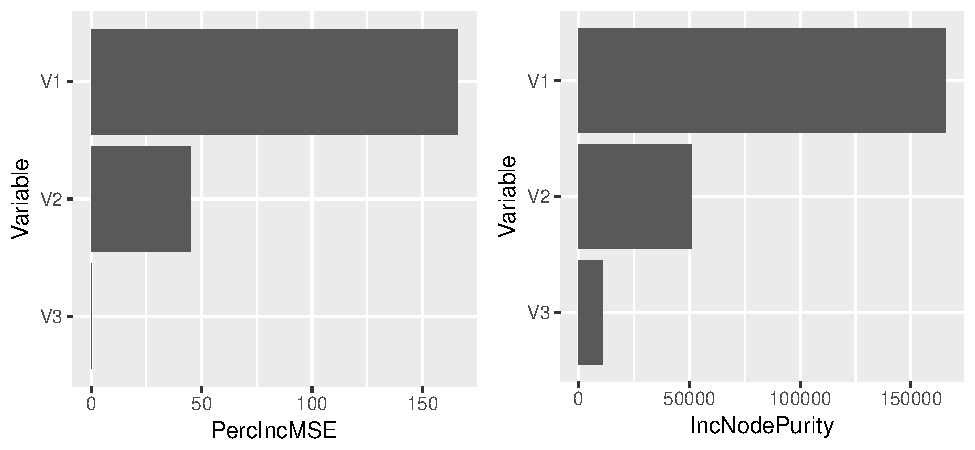
\includegraphics{thesis_files/figure-latex/unnamed-chunk-3-1.pdf}
\caption{\label{fig:unnamed-chunk-3}\label{mda_ex}Example of MDA and MDI
Variable Importance}
\end{figure}
Note that for both variable importance measures, the contribution of
each predictor is properly captured. That is, \(X_1\) is the most
important variable followed by \(X_2\), with \(X_3\) having no
contribution with the MDA importance measure. With MDI, the contribution
of \(X_3\) is non-zero likely due to the randomization introduced in the
splitting variable step.

\subsection{Issues with Random
Forests}\label{issues-with-random-forests}

While random forests are good out of the box predictors, there are
situations where the random forest algorithm can fail to produce good
predictions. If the underlying regression function is linear, if the
predictors are highly correlated, or if the data cannot be bootstrapped,
then the random forest will not perform well. Relative to other methods,
random forests are especially adept at handling highly non-linear
functions, but can struggle with linear response compared to say linear
regression. \par

If the predictors are highly correlated, then it has been shown by
Strobl, Boulesteix, Zeileis, \& Hothorn (2007) and Strobl, Boulesteix,
Kneib, Augustin, \& Zeileis (2008) that the trees within the forest
ensemble will be biased and the variable importance measures will not be
reliable due to confounding between similar looking variables. While the
randomization step in the random forest algorithm can alleviate the
correlation between trees in the ensemble, the collinearity between
predictors can cause the predictive performance of the random forest to
suffer. This is an issue with the underlying CART algorithm. Alternative
algorithms from CART exist which try to alleviate issues of collinearity
and correlation in predictors, but we focus primarily on the forest
ensembles grown using CART in this thesis. \par

Finally, there are situations where the data cannot be bootstrapped.
This could be due to a number of factors including that the data has a
heavily-tailed distribution or if there are particularly extreme values.
In this case, a different bootstrap scheme could perhaps remedy the
situation where the naive bootstrap fails. One common resampling scheme
used within random forests is to use the m-out-of-n bootstrap (also
referred to subsampling or subagging in the literature). The m-out-of-n
bootstrap is a resampling scheme which resamples with or without
replacement \(m\leq n\) observations from the data to form datasets with
\(m\) many data points to run the bootstrap computation. Of course,
using less of the available data is less efficient, but in the context
of random forests this loss of efficiency may not be an issue. In Strobl
et al. (2008), simulation results showed that subsampling instead of
using the standard nonparametric bootstrap can improve the performance
of random forests. The authors suggested that subsampling further
reduces the variance of the ensemble by producing trees that are even
more decorrelated. Their heuristic is that there is a lower probability
of duplicate data points being chosen using subsampling (this
probability is zero if we are subsampling without replacement),
furthermore there is a lower probability of highly correlated data
points being chosen as one of the \(m\leq n\) points. This certainly
seems plausible, but we would like to see further simulation results or
a technical result that explains why subsampling works well for forests.
We would also like to note that consistency results such as from Mentch
\& Hooker (2016b) and Wager \& Athey (2017) make this subsampling
assumption in their analysis of the random forest model, as subsampling
constructions make the forest ensemble more amenable to mathematical
analysis. \par

\section{Focus of this Thesis}\label{focus-of-this-thesis}

An issue with random forest variable importance measures is bias due to
the presence of correlated predictors. As will become clearer in the
next chapter, correlated predictors can lead to unreliable MDA and MDI
variable importance scores due to confounding between correlated
predictors. The weakness of commonly used random forest variable
importance measures to correlated predictors is unfortunate as random
forests often produce good predictions with little tuning required
except growing a sufficient number of trees and choosing a good value of
\(m\leq p\) to try at each split in the tree growing process. The ease
of fitting random forests is one of the advantages of the random forest
algorithm compred to more complex methods like neural networks or
support vector machines. Since the random forest algorithm is a readily
available and easy to use tool for statistical practitioners, we would
like to develop random forest variable importance measures which can
take into account correlated predictors. Our goal with this thesis is
to:
\begin{enumerate}
  \item Develop computationally tractible random forest variable importance measures which can handle correlated predictors in the data. 
  \item Extend our random forest variable importance measures to a hypothesis testing framework via permutation tests. 
  \end{enumerate}
\par

\chapter{Variable Importance and Inference for Random
Forests}\label{variable-importance-and-inference-for-random-forests}

\section{Introduction}\label{introduction-1}

In this chapter we focus on approaches of inference for random forests
involving variable importance measures of random forests. Such
approaches involve using variable importance measures of random forests
to evaluate the relative importance of different variables in the
construction of the forest. Louppe (2014) and Ishwaran (2007) focused on
theoretical properties of variable importance measures while Owens
(2017), Strobl et al. (2007), and Strobl et al. (2008) are centered on
developing less biased variable importance measures for hypothesis
testing. \par

\section{Theoretical Analysis of MDA Variable Importance
Measures}\label{theoretical-analysis-of-mda-variable-importance-measures}

The approach to variable importances adopted in Ishwaran (2007) differs
from the original variable importance measures for random forests, so we
require some additional vocabulary. \par 

Suppose \(T\) is a binary recursive tree and suppose that \(T\) has
\(M\) many terminal nodes. For each point \(\mathbf{x}\) in the feature
space, \(T\) maps \(\mathbf{x}\) to one of the \(M\)-many terminal
nodes. In particular, if we let \(\mathcal{X}\) denote the feature
space, then \(T\) is a function
\(\mathcal{X}\rightarrow \{1,\ldots, M\}\) defined by the equation
\[T(\mathbf{x})=\sum_{m=1}^M m B_m(\mathbf{x}),\] where
\(B_m(\mathbf{x})\) is a \(0-1\) basis function which partition the
feature space \(\mathcal{X}\). \par

Let \(Z=\{(\mathbf{x}_i,Y_i)|i=1,\ldots,n\}\) denote the training data,
where \(\mathbf{x}_i\) is a covariate in the feature space and \(Y_i\)
is the response. We call \(T\) a binary regression tree if it is a
binary recursive tree grown from \(Z\) using using binary recursive
splits of the form \(x_j\leq c\) and \(x_j> c\) where split values \(c\)
are chosen based on the observed \(\mathbf{x}_i\) in the training data
\(Z\). The value \(a_m\) in the terminal node is the average response of
the training observations falling in the \(m\)th node. That is,
\[a_m=\frac{\sum_{i=1}^n \mathbb{I}\{T(\mathbf{x}_i)=m\} Y_i}{\sum_{i=1}^n \mathbb{I}\{T(\mathbf{x}_i)=m\}}.\]
Note that \(\mathbf{x_i}\) denotes a row of covariates for the training
data \(Z\), while \(x_j\) denotes the \(j\)th variable along the columns
of the training data. \par

For a binary regression tree, the basis functions \(B_m(\mathbf{x})\)
are product splines of the following form:
\[B_m(\mathbf{x})=\prod_{l = 1}^{L_m} [x_{l(m)}-c_{l, m}]_{s_{l,m}},\]
where \(L_m\) denotes the number of splits used to construct
\(B_m(\mathbf{x})\). For each split \(l\), there is a splitting variable
\(\mathbf{x}_{l(m)}\) which denotes the \(l(m)\)th coordinate of
\(\mathbf{x}\) and a splitting value \(c_{l,m}\). The \(s_{l,m}\) are
binary \(\pm 1\) values, where for a given scalar \(x\),
\([x]_{+1}=\mathbb{I}(x>0)\) and \([x]_{-1}=\mathbb{I}(x\leq 0).\) Note
that the basis functions satisfy an orthogonality property, which gives
\(B_m(\mathbf{x})B_{m'}(\mathbf{x})=0\) if \(m\neq m'\). Note also that
given a tree \(T\), the predictor associated with the tree can be
written as a linear combination of basis functions:
\[\hat{\mu}(\mathbf{x})=\sum_{m=1}^M a_m B_m(\mathbf{x}).\] We are now
prepared to define Ishwaran's variable importance measure. \par

Informally, the \(MDA\) variable importance of a variable \(x_j\) is the
difference between \(MSE\) of the tree \(T\) when \(x_j\) is randomly
permuted and \(MSE\) of the tree \(T\) when \(x_j\) is not permuted. As
such a scheme of variable importance is difficult to analyze, Ishwaran
proposes a surrogate measure. For the variable \(x_j\), we drop
\(\mathbf{x}\) down the tree and follow the binary splits until either a
terminal node is reached or a node with a split depending on \(x_j\) is
reached. If a node with a split depending on \(x_j\) is reached, we then
subsequently assign \(\mathbf{x}\) randomly to either the left or right
daughter node, whenever there is a split, until we reach a terminal
node. The difference in \(MSE\) between noising up \(x_j\) and not
noising up \(x_j\) to be the variable importance of \(x_j\) in the tree
\(T\). Denote the tree that results from noising up \(x_j\) by \(T_j\).
\par

Such a scheme relies on the following heuristic: if we chose an adequete
splitting rule to construct our tree, then we expect that variables that
are split earlier in the tree are more important, since prediction will
suffer the most from noising up a variable higher up in the tree than a
variable close to a terminal node. This is a behavior observed in CART
trees and random forests based on CART: splits closer to the root node
are more influential than splits close to terminal nodes, so the MDA or
MDI variable importance of variables split on close to the root node are
expected to be higher than otherwise. \par

\subsection{Maximal Subtrees and Theoretical
Results}\label{maximal-subtrees-and-theoretical-results}

Defining a structure on binary regression trees called subtrees, we can
write the predictor for the noised up tree as a deterministic component
relying on terminal nodes for no parent nodes involve a split on
\(x_j\), and a random component involving terminal nodes for which there
are parent nodes involving a split on \(x_j\). The definition of the
subtree is quite intuitive. We call \(\tilde{T}_j\) a \(j\)-subtree of
the tree \(T\), if the root node of \(\tilde{T}_j\) has daughters that
depend on an \(x_j\) split. A \(j\)-subtree \(\tilde{T}_j\) is a maximal
\(j\)-subtree of the tree \(T\), if there are no larger \(j\)-subtrees
continaing \(\tilde{T}_j\). For a given tree \(T\) and for each variable
\(x_j\), there is a set of \(K_j\) many distinct maximal \(j\)-subtrees,
which are denoted by \(\tilde{T}_{1,j},\ldots, \tilde{T}_{K_j,j}\). Note
each distinct \(\tilde{T}_{k,j}\) maximal \(j\)-subtree contains a set
of distinct terminal nodes \(M_{k,j}\). Each \(M_{k,j}\) is distinct for
\(k=1,\ldots,K_j\), since we are working with maximal \(j\)-subtrees.
Define \[M_j=\bigcup_{k=1}^{K_j} M_{k,j}\] to be the set of terminal
nodes for which there is a parent node involving a split on \(x_j\).
Ishwaran (2007) proves the following lemma about the functional form of
the predictor for the tree \(T_j\). \par
\begin{lemma}
Let $\hat{\mu}_j(\mathbf{x})$ denote the predictor for $T_j$. Then $$\hat{\mu}_j(\mathbf{x})=\sum_{m\notin M_j}a_m B_m(\mathbf{x})+\sum_{k=1}^{K_j} \tilde{a}_{k,j}\mathbb{I}\{T(\mathbf{x})\in M_{k,j}\},$$ where $\tilde{a}_{k,j}$ is the random terminal value assigned by $\tilde{T}_{k,j}$ under the random left right path through $\tilde{T}_{k,j}$. We write $\tilde{P}_{k,j}$ to denote the distribution of $\tilde{a}_{k,j}$. 
\end{lemma}
For a proof, see Ishwaran (2007). It is a bit surprising that the
functional form of \(\hat{mu}_j(\mathbf{x})\) can be separated into the
two components. Given this lemma and the definition of \(j\)-subtrees,
we can more formally define the variable importance of \(x_j\) in the
tree \(T\). \par

Let \(g\) be a loss function. Often we use the squared error to evaluate
loss, which corresponds to \(MSE\), but there is no strict requirement
in the definition. Denote the test data by \((Y,\mathbf{x})\). Then the
prediction error of the predictor \(\hat{\mu}\) is given by
\(\mathbb{E}(g(Y,\hat{\mu}(\mathbf{x})))\). As a reminder, we assume
that there is an underlying regression function
\[Y=\mu(\mathbf{x})+\varepsilon,\] where \(\varepsilon\) is independent
error with zero mean and variance \(\sigma^2>0\). Similarly, we can
define the prediction error of the predictor \(\hat{\mu}_j\) to be
\(\mathbb{E}(g(Y,\hat{\mu}_j(\mathbf{x}))).\) Set
\(g(Y,\hat{\mu}(\mathbf{x}))=(Y-\hat{\mu}(\mathbf{x}))^2\) to be the
\(L_2\) loss, which corresponds to \(MSE\). Define the variable
importance of the variable \(x_j\) to be
\[\Delta_j=\mathbb{E}((Y-\hat{\mu}_j(\mathbf{x}))^2)-\mathbb{E}((Y-\hat{\mu}(\mathbf{x}))^2).\]
Application of the lemma and some manipulation allows us to write
\[\Delta_j=\mathbb{E}(R_j(\mathbf{x})^2)-2\mathbb{E}\left(R_j(\mathbf{x})[\mu(\mathbf{x})-\hat{\mu}(\mathbf{x})]\right),\]
where
\[R_j(\mathbf{x})=\sum_{k=1}^{K_j}\sum_{m\in M_{k,j}} (\tilde{a}_{k,j} -a_m)B_m(\mathbf{x}).\]
\par

As noted in Ishwaran (2007), we make the assumption that the true
regression function \(\mu\) is of similar form to \(T\). That is, assume
\[\mu(\mathbf{x})=\sum_{m=1}^M a_{m,0} B_m(\mathbf{x}),\] where
\(a_{m,0}\) are the true, but unknown, terminal values. Under this and
some other large sample assumptions, Ishwaran finds that asymptotically,
each maximal \(j\)-subtree will tend to contribute equally to the
variable importance \(\Delta_j\). In effect, nodes closer to the root of
a maximal \(j\)-subtree will have a larger effect on \(\Delta_j\) than
nodes closer to the terminal nodes. \par

\subsection{Extension to Forest
Ensembles}\label{extension-to-forest-ensembles}

The framework developed in Ishwaran (2007) extends naturally to forest
ensembles and his theoretical result regarding forest ensembles provides
some information of the behavior of variable importance measures for
random forests. First for some notation, recall that in the forest
ensemble setting, we draw \(B\) many bootstrap resamples of the training
data to obtain the bootstrap replicates
\(Z^{b}=\{(\mathbf{x}_i^b, Y_i^b)|i=1,\ldots,n\}\) of the training data
for \(b=1,\ldots, B\). We then construct a binary regression tree
\(T(\mathbf{x};b)\) on each bootstrap replicate of the data and have the
forest \(\hat{\mu}_F\) as the average of predictions over the trees
\(T(\mathbf{x};b)\):
\[\hat{\mu}_F(\mathbf{x})=\frac{1}{B}\sum_{b=1}^B \hat{\mu}(\mathbf{x};b),\]
where \(\hat{\mu}(\mathbf{x};b)\) denotes the predictor for the tree
\(T(\mathbf{x};b)\). Given that each \(\hat{\mu}(\mathbf{x};b)\) is a
linear combination of basis functions, we can write
\[\hat{\mu_F}(\mathbf{x})=\frac{1}{B}\sum_{b=1}^B\sum_{m=1}^{M^b}a_m^b B_m(\mathbf{x};b).\]
Again assume that the \(\mu(\mathbf{x})\) has a similar structure to
\(\mu(\mathbf{x})\). That is,
\(\mu(\mathbf{x})=\frac{1}{B}\sum_{b=1}^B\sum_{m=1}^{M^b}a_{m,0}^b B_m(\mathbf{x};b)\),
where \(a_{m,0}\) are the true, but unknown, terminal values. We denote
the noised up forest predictor for the variable \(x_j\) by
\(\hat{\mu}_{F_j}(\mathbf{x})\). As with the normal forest predictor,
the noised up forest predictor is the average of the noised up
predictors \(\hat{\mu}_j\) over the bootstrap resamples:
\[\hat{\mu}_j(\mathbf{x})=\sum_{b=1}^B \hat{\mu}_j(\mathbf{x};b).\] As
forest predictors are simply the average of individual trees, we can
extend the lemma to \(\hat{\mu}_{F_j}\) with the use of \(b\)'s in
appropriate places denoting the usage of the \(b\)th bootstrap resample.
That is, we can write
\[\hat{\mu}_{F_j}(\mathbf{x})=\frac{1}{B}\sum_{b=1}^B\left(\sum_{m\notin M_j^b} a_m^b B_m(\mathbf{x};b)+\sum_{k=1}^{K_j^b} \tilde{a}_{k,j}^b \mathbb{I}\{T(\mathbf{x};b)\in M_{k,j}^b\} \right).\]
The variable importance of the variable \(x_j\) is defined to be
\[\Delta_{F_j}=\mathbb{E}((Y-\hat{\mu}_{F_j}(\mathbf{x}))^2)-\mathbb{E}((Y-\hat{\mu}(\mathbf{x}))^2).\]
Similar to the single tree case, the variable importance of the variable
\(x_j\) in the forest ensemble can be written as
\[\Delta_{F_j}=\mathbb{E}(R_{F_j}(\mathbf{x})^2)-2\mathbb{E}\left(R_{F_j}(\mathbf{x})[\mu(\mathbf{x})-\hat{\mu}_F(\mathbf{x})]\right),\]
where
\[R_{F_j}(\mathbf{x})=\frac{1}{B}\sum_{b=1}^b\sum_{k=1}^{K_j^b} \sum_{m\in M_{k,j}^b} (\tilde{a}_{k,j}^b-a_m^b)B_m(\mathbf{x}; b).\]
\par

We are now ready to state a result about the asymptotic form of
\(\Delta_{f,j}\):
\begin{theorem}
Let $R_{F_j, 0}(\mathbf{x})$ be the function $R_{F_j}(\mathbf{x})$, in which each instance of $a_m^b$ has been replaced with $a_{m,0}^b$. Assume that $Y$ can be written in terms of a regression model $$Y=\mu(\mathbf{x})+\varepsilon$$ and that $$\mu(\mathbf{x})=\frac{1}{B}\sum_{b=1}^B\sum_{m=1}^{M^b}a_{m,0}^b B_m(\mathbf{x};b).$$ If $a_m^b\rightarrow a_{m,0}^b$ for each $m$ and $b$, then $$\Delta_{F_j}\rightarrow \mathbb{E}\left(R_{F_j,0}(\mathbf{x})^2\right)\leq\mathbb{E}\left(\frac{1}{B}\sum_{b=1}^b\sum_{k=1}^{K_j^b}\theta_0(k,j,b)\right),$$ where $$\theta_0(k,j,b)=\sum_{m\in M_{k,j}^b} \pi_{m,b}\tilde{P}_{k,j,0}^b\left(\tilde{a}_{k,j,0}^b-a_{m,0}^b\right)^2$$ is the node mean squared error for the $k$th maximal $v$-subtree of $T(\mathbf{x};b)$and $\pi_{m,b}=\mathbb{P}(B_m(\mathbf{x};b)=1|Z)$. 
\end{theorem}
For a proof, see Ishwaran (2007). As Ishwaran (2007) notes, the bound in
the above theorem becomes tighter as the trees in the forest become more
and more orthogonal to each other. The above theorem is applicable if
the forest predictor is consistent. This suggests that forest ensemble
methods which are consistent and produce trees that are at least
approximately orthogonal to each other allow for variable importance to
be characterized through node mean squared error of subtrees. Variable
importance as defined above differs from the \(MDA\) variable importance
for random forests, but the two follow a similar heuristic towards
measuring variable importance via the loss of predictive accuracy when
the variable \(x_j\) is pertrubed. Therefore this result suggests that,
perhaps, so long as the random forest estimator is consistent and the
trees constructed are at least approximately orthogonal, the \(MDA\)
variable importance can be characterized via the mean squared error of
some analogous structure to maximal subtrees. This is, of course,
conjectural, but we are interested whether for simpler forest
algorithms, results similar to the theorem can be proven. Asymptotic
results for the \(MDA\) and also \(MDI\) variable importance measures
are difficult to formulate and prove for several reasons. First, the
\(CART\) tree construction process combined with the bootstrapping and
randomization procedure of the random forest is difficult to
mathematically analyze. Second, it is still unknown whether random
forests constructed via \(CART\) are consistent. However, there are
other random forest variants known to be consistent, so those variants
may be a natural starting point to try to prove asymptotic results about
\(MDA\) and \(MDI\) variable importances. Third, the definition of
\(MDA\) variable importance involves a permutation step that is
difficult to analyze mathematically. The above results are
mathematically amenable due to the noising-up procedure adopted allowing
for a quite elegant analysis of the variable importance. One possible
approach to dealing with this issue may be to adopt the above definition
of variable importance in different random forest settings and see if
similar results to Ishwaran (2007) may be derived. Another approach,
which is the one more or less taken by Ishwaran (2007), is to to find a
mathematically tractible definition of variable importance which is
approximately the MDA variable importance measure and proceed with
analysis from there. \par

\section{Theoretical Analysis of MDI Variable
Importance}\label{theoretical-analysis-of-mdi-variable-importance}

Up to now in this chapter, we have been discussing theoretical results
concerning the \(MDA\) variable importance. Louppe (2014) has explored
some of the theory for \(MDI\) variable importance of forest ensembles.
\par

In order to discuss the following theoretical results regarding MDI
variable importance, we make some modifications to the setting we are
working in. Assume that we are working in a finite probability space
{[}this assumption is necessary primarily for technical reasons{]} and
that observations \(Y,X_1,\ldots,X_p\) in the training set \(Z\) are
categorical variables. Recall that if a forest ensemble is grown by
choosing splits and variables maximizing the decrease in nodal impurity
where \(i(s,t)\) denotes the impurity measure used, then the MDI
variable importance of the variable \(X_j\) is defined to be
\[VI(X_j)=\frac{1}{B}\sum_{b=1}^B \sum_{t\in T_b} \mathbb{I}(j_t=j)p(t)\Delta i(s,t),\]
where \(p(t)\) is the proportion of samples which reach the node \(t\)
in the tree \(T_b\). Note that MDI variable importance is the average
over the bootstrap resamples of the sum of the weighted decrease in
impurity over the nodes of the tree using \(X_j\) as the splitting
variable. \par

Rather than working with random forests, we will work with an infinite
ensemble of totally randomized and fully developed trees. Totally
randomized and fully developed trees are a variant of forest ensembles
given by the following. A totally randomized and fully developed tree is
a decision tree in which each node \(t\) is partioned using a variable
\(X_j\) picked uniformly at random among those not yet used at the
parent nodes of \(t\), where each node \(t\) is split into \(|X_j|\)
sub-trees, i.e., one for each possiblevalue of \(X_j\), and where the
recursive construction process halts only when all \(p\) variables have
been used along the current branch. \par

Using an impurity measure called Shannon entropy, Louppe (2014) is able
to show that only relevant variables (that is variables whose
information content, conditional on the other variables, is useful
towards explaining the response \(Y\)) have non-zero infinite sample
size variable importance. Furthermore, this means that irrelevant
variables (which are variables whose information content, conditional on
the other variables, is not useful towards explaining the response
\(Y\)) have a infinite sample size variable importance of zero. In fact,
in this context, a variable is irrelevant if and only if it has an
infinite sample size variable importance of zero. Generalizing from
Shannon entropy to other impurity measures, for the GINI index (used in
commonly in classification problems) and variance (used in regression
via MSE), only irrelevant variables result in no decrease in nodal
impurity. We would like to reiterate that these results concerning
irrelvant variables are valid particularly in the setting of infinite
ensembles of totally randomized and fully developed trees. \par

In the random forest setting, the results discussed in the previous
paragraph may not be valid. In the random forest setting, a key step in
the construction of trees is the randomization step in which we choose
at random a subset of size \(m\leq p\) of the variables to choose the
next split from. If \(m>1\), then it is possible for some variables to
never be chosen at a node \(t\), since there will always be other
variables which have a larger decrease in nodal impurity. This results
in trees in which the variables with the largest reduction in nodal
impurity are centered in the trunk of the tree with variables with
smaller reduction in nodal impurity are pushed to leaves, or otherwise
not chosen to split on. This is an undesirable property to have since
this can result in an ensemble which inadequately explores the feature
space and is thus more consistently biased towards some variables over
others, even if other variables can provide only slightly lower
reductions in nodal impurity. As a consequence, if \(m>1\), then it is
not the case that a variable is irrelevant if and only if it has a
variable importance of zero. One implication is that in data sets where
there are correlated variables, random forest variable importance
measures may result in variable importances which do not reflect the
actually importance of variables in explaining the response \(Y\). In
particular, it could be the case that if \(X_j\) and \(X_{j'}\) are two
correlated variables, then even if both \(X_j\) and \(X_{j'}\) are
important in explaining the response \(Y\), it may be the case that
\(X_j\) is consistently chosen as the splitting variable over \(X_{j'}\)
if the two variables are both possible splitting variables. \par

\section{Dealing with Bias in Random Forest Variable
Importance}\label{dealing-with-bias-in-random-forest-variable-importance}

In the previous two sections of this chapter we discussed theoretical
results pertaining to MDA and MDI variable importance measures. For MDA
variable importance, a consistent ensemble with orthogonal trees have a
nice asymptotic form in the framework developed in Ishwaran (2007). On
the otherhand, with MDI variable importance, if the trees are grown in
the random forest setting, then there are issues of the variable
importance not capturing the actual importance of the variables in the
training data. This could particularly arise as an issue in data sets
with correlated variables where equally important variables receive
different variable importances due to bias introduced by tree
construction process. In using the term `bias,' we would like to
emphasise that this is not bias in the sense of biased estimators, but
bias in the sense of which variables are chosen to be split upon in the
tree growing process. Bias in the variable importance measures of random
forests is concerning as we would like to be able to use random forests
for inferential statistics. A couple of methods have been proposed to
construct more reliable variable importance measures, which we discuss
in this section. \par

\subsection{Bias in Random Forest Variable Importance
Measures}\label{bias-in-random-forest-variable-importance-measures}

Bias in random forest variable importance measures was first
substantively analyzed in Strobl et al. (2007). Strobl et al. (2007) ran
a simulation study comparing MDI variable importance using the GINI
index, MDA variable importance, and a conditional variable importance
measure in a classification setting. The conditional variable importance
measure used by Strobl et al. (2007) is a variable importance method
similar to MDA variable importance, but utilizing an ensemble of
conditional inference trees. We will define conditional inference trees
and the conditional variable importance measures below. For now, note
that Strobl et al. (2007) found that MDI variable importance using the
GINI index and MDA variable importance tends to be biased from the
expected variable importance value within their simulation. They also
found that subsampling without replacement tends to reduce the bias in
variable importance in comparison to using bootstrap resampling with
replacement. In their analysis, Strobl et al. (2007) claim that the GINI
index tends to favor variables with more potential cutpoints. Hence the
MDI variable importance measure using the GINI index is biased towards
variables with more potential cutpoints. Strobl et al. (2007) also found
that in using the MDA variable importance measure, since variables that
are split upon closer to the root node affect the predictive accuracy of
the ensemble more than variables split upon in leaves, the MDA variable
importance measure will be affected by the variable selection bias of
individual trees. Furthermore, Strobl et al. (2008) find that correlated
variables tend to be overselected in the tree growing process. In order
to utilize random forest variable importance measures as inferential
tools, several methods have been proposed to deal with the issue of
variable selection bias in random forests.

\subsection{Conditional Variable
Importance}\label{conditional-variable-importance}

The MDA variable importance measure can be viewed in the context of
permutation tests and hypothesis testing. In particular, we can consider
that the MDA variable importance measure operates on the null hypothesis
that permuting the values of the variable \(X_j\) has no affect on the
predictive accuracy of the random forest predictor. This corresponds to
the null hypothesis that the variable \(X_j\) is independent of the
response \(Y\) and the variables \(X_1,\ldots,X_p\). If the predictive
accuracy of the random forest suffers from permuting \(X_j\), that is if
the \(VI(X_j)\) is nonzero, then if also \(X_j\perp X_{-j}\), it would
follow that \(Y\) and \(X_j\) are not independent. However, it is
important to note that the null hypothesis under which the MDA variable
importance measure operates is: \[H_0:X_j \perp Y,X_{-j}.\] If on the
otherhand, \(X_j\) and \(X_{-j}\) are not independent, then \(VI(X_j)\)
will be biased by the correlation between \(X_j\) and \(X_{-j}\). It
could be that \(Y\) and \(X_j\) are not independent or that \(Y\) and
\(X_j\) are independent, but in either case, if the predictor variables
are correlated, we see that \(VI(X_j)\) will not accurately capture the
importance of \(X_j\). Strobl et al. (2008) propose a permutation scheme
corresponding to the null hypothesis \[H_0:(X_j\perp Y)|X_{-j},\] that
is that \(X_j\) is independent of \(Y\) conditional on the \(X_{-j}\).
Such a permutation scheme would take into account the correlation
structure of the predictor variables and would allow for a less biased
variable importance measure so long as the individual trees within the
ensembles do not exhibit large variable selection bias. \par

Strobl et al. (2008) propose defining a grid within which values of
\(X_j\) are permuted according to partitions of the feature space given
by each tree. While Strobl et al. (2008) propose using unbiased
conditional inference trees from Hothorn, Hornik, \& Zeileis (2006) to
determine the partition, it is possible to use partitions given by CART
trees. The algorithm is presented as follows. \par
\begin{algorithm}
    \caption{Conditional Variable Importance} \label{conditional variable importance}
      \begin{algorithmic}[1]
        \State Grow a forest ensemble $\{T_b\}_{b=1}^B$
          \For{ $j=1,\ldots,p$ }
            \For{ $b=1,\ldots,B$ }
            \State Compute $RSS(T_b,Z_b)$.
            \For{ all variables $X_i$ to be conditioned on }
            \State Extract cutpoints that split $X_i$ in the tree $T_b$ and create a grid $\mathcal{G}$ by bisecting the sample space in each cutpoint.
            \EndFor
            \State Within the grid $\mathcal{G}$, permute the values of $X_j$ and denote the permuted resample by $Z_b^j$.
            \State Compute $RSS(T_b,Z_b^j)$.
            \State Compute the conditional variable importance of $X_j$ in the tree $T_b$ to be $VI_b(X_j)=\frac{1}{|Z_b|}\left(RSS(T_b,Z_b)-RSS(T_b,Z_b^j)\right)$.
            \EndFor
            \State Compute the conditional variable importance of $X_j$ in the forest ensemble to be $VI(X_j)=\frac{1}{B}\sum_{b=1}^B VI_b(X_j)$.
          \EndFor
      \end{algorithmic}
  \end{algorithm}
To determine the variables \(X_i\) to be conditioned on Strobl et al.
(2008) suggest including only variables whose empirical correlation with
the variable \(X_j\) suggests some reasonable threshold. \par

\subsection{Infforest Variable
Importance}\label{infforest-variable-importance}

While simulation results of Strobl et al. (2008) suggest that the
conditional variable importance is more effective at capturing the
importance of each variable \(X_j\) compared to the marginal approach
followed in MDA, they note that conditional variable importance cannot
completely eliminate preference for correlated variables in random
forests. Owens (2017) instead suggests a partition then permute scheme
which produces a sampling distribution for the variable importance of
each variable \(X_j\). Once a sampling distribution for \(VI(X_j)\) has
been obtained, hypothesis testing and other sorts of statistical
inference can proceed. As the Infforest variable importance is quite
complicated, some explanation is needed. \par

After growing a forest ensemble \(\{T_b\}_{b=1}^B\), infforest variable
importance values are computed as follows. First, for each
\(b=1,\ldots,B\) and each variable \(X_j\), grow a tree
\(X_j\sim X_1,\ldots,X_{j-1},X_{j+1},\ldots,X_p\) using all \(p-1\)
predictors using the in-bag sample used to grow \(T_b\). Denote this
tree by \(T_j^{b*}\). The rows of \(\overline{Z}_b\) are permuted within
the partitions of the feature space determined by \(T_j^{b*}\). The
difference in predictive accuracy of \(T_b\) before and after the OOB
sample \(\overline{Z}_b\) has been permuted is the infforest variable
importance for the variable \(X_j\) in the tree \(T_b\). Owens (2017)
suggests then using the sampling distribution of \(VI(X_j)\) obtained
from the infforest partition-permute scheme to test the null hypothesis
that the variable importance of \(X_j\) is zero. On the other hand, if
we let \(VI_b(X_j)\) denote the infforest variable importance of the
variable \(X_j\) in the tree \(T_b\), then we could define the infforest
variable importance of \(X_j\) in the forest ensemble
\(\{T_b\}_{b=1}^B\) to be \[VI(X_j)=\frac{1}{B}\sum_{b=1}^B VI_b(X_j).\]
In particular, this corresponds to the mean of the sampling distribution
of the infforest variable importances of \(X_j\) over the trees \(T_b\).
\par

Originally, Owens (2017) developed for random forests using CART trees
as base learners. However, the infforest variable importance could
certainly be used with random forest variants such as conditional
inference forests used in Strobl et al. (2008). Another possible
modification of the infforest variable importance algorithm is to only
grow an auxilary tree predicting
\(X_j\sim X_{\alpha_1},\ldots,X_{\alpha_k}\), where
\(X_{\alpha_1},\ldots,X_{\alpha_k}\) are variables whose correlation
with \(X_j\) exceeds some reasonable threshold. This would combine the
suggestion in Strobl et al. (2008) of considering the correlation
structure of the predictor variables in setting up the grid for the
conditional variable importance with the infforest partition-permute
scheme. \par

One issue with infforest variable importance is the steep computational
cost of the algorithm. The algorithm grows an auxilary tree
\(T_{j}^{b*}\) for each variable \(X_j\) and bootstrap resample \(b\)
and then proceeds to permute the OOB sample with respect to each
\(T_j^{b*}\). Even implementing the infforest variable importance
algorithm on small bootstrap resamples of around several hundred is
computationally intensive. \par
\begin{algorithm}
    \caption{Infforest Variable Importance} \label{infforest variable importance}
      \begin{algorithmic}[1]
        \State Grow a forest ensemble $\{T_b\}_{b=1}^B$
          \For{ $j=1,\ldots,p$ }
            \For{ $b=1,\ldots,B$ }
              \State Compute $RSS(T_b,\overline{Z}_b)$.
              \State Grow a tree $T_j^{b*}$ predicting $X_j\sim X_{-j}$ using in-bag sample.
              \State Permute rows of the OOB sample $\overline{Z}_b$ with respect to the partitions of the feature space from $T_j^{b*}$ to obtain the permuted OOB sample $\overline{Z}_b^*$. 
              \State Compute $RSS(T_b,\overline{Z}_b^*)$.
              \State Compute the infforest variable importance of $X_j$ in $T_b$ to be $VI_b(X_j)=\frac{1}{\overline{Z}_b}\left(RSS(T_b,\overline{Z}_b)-RSS(T_b,\overline{Z}_b^*)\right)$.  
            \EndFor
            \State Test the null hypothesis that the variable importance of $X_j$ is zero using the distribution of values $VI_b(X_j)$. 
          \EndFor
      \end{algorithmic}
  \end{algorithm}
\chapter{Added Variable Plot
Importance}\label{added-variable-plot-importance}

\section{Introduction}\label{introduction-2}

In the previous chapter, we discussed theoretical properties and
observed behavior of random forest variable importance measures. In
particular, we discussed issues of bias present in the MDA variable
importance measure. Strobl et al. (2008) and Owens (2017) proposed the
conditional variable importance measure and the Infforest variable
importance measures, respectively, as methods of accounting for bias in
variable selection among correlated predictors when measuring variable
importance in a forest ensemble. Conditional variable importance and
Infforest variable importance aim at measuring the conditional
importance of a particular variable by conditionally permuting OOB data
according to some criteria measured from the data, whether that be
empirical correlation in the case of conditional variable importance, or
the partitions induced by a particular tree inthe case of Infforest
variable importance. In any case, we are primarily interested in the
conditional importance of a predictor given the information provided by
other predictors. While we would like to have a exact method of
computing the conditional importance of a predictor in a random forest
ensemble, in practice it is unclear how to construct an exact method
given the complexity of the random forest ensemble. We can, however,
estimate the effect of adding a predictor to the set of predictors that
the forest ensemble can split on via a type of diagnostic plot called an
added variable plot. \par

Added variable plots are a diagnostic plot which estimate the effect of
adding a predictor variable to the model. In this chapter we propose a
method of measuring the importance of each predictor in a random forest
ensemble via a quantity we call the Added Variable Importance (AVI) that
depends on the added variable plot of each predictor. The AVI attempts
to estimate the effect of adding a predictor as a possible candidate in
the splitting step of the random forest ensemble. To understand AVI, we
regress from the random forest setting to the linear regression setting
to explain how added variable plots work. \par

\section{Added Variable Plots in Linear
Regression}\label{added-variable-plots-in-linear-regression}

Suppose that we have data \(Z=\{(\mathbf{x}_i,Y_i)|i=1,\ldots,n\}\),
where \(\mathbf{x}_i\) is a covariate in the feature space, and that we
fit a multiple linear regression model of the form
\[\mathbf{Y}_1=\mathbf{X}\beta_1+\mathbf{W}\alpha+\mathbf{\varepsilon}_1\]
where \(\mathbf{X}\) is a \(n\times p\) matrix consisting of \(p-1\)
predictors, \(\beta=(\beta_0,\beta_1,\ldots,\beta_p)^T\),
\(\mathbf{W}=(w_1,\ldots,w_n)\) is a predictor, \(\alpha\) is a scalar,
and \(\text{Var}(\mathbf{\varepsilon})=\sigma^2 I\). \par

Say we are interested in estimating the effect of the predictor
\(\mathbf{W}\) in the regression model \(\hat{\mathbf{Y}}_1\). We could
first fit the models \(\hat{\mathbf{Y}}_2=\mathbf{X}\beta_2\) and
\(\hat{\mathbf{W}}=\mathbf{X}\delta\), where \(\beta_2\) and \(\delta\)
are coefficient vectors like \(\beta_1\) and then plot the residuals
\(\mathbf{W}-\hat{\mathbf{W}}\) against the residuals
\(\mathbf{Y}-\hat{\mathbf{Y}}_2\). The plot we obtain by plotting
\(\mathbf{W}-\hat{\mathbf{W}}\) against
\(\mathbf{Y}-\hat{\mathbf{Y}}_2\) is called the added variable plot of
\(\mathbf{W}\) and measures the effect of \(\mathbf{W}\) on
\(\mathbf{Y}\) once we have adjusted for the effect of \(\mathbf{X}\) on
\(\mathbf{W}\) and \(\mathbf{Y}\), respectively. In particular, the
residuals that we plot for the added variable plot is the portion of
\(\mathbf{W}\) unexplained by \(\mathbf{X}\) on the \(x\)-axis and the
portion of \(\mathbf{Y}\) unexplained by
\(\hat{\mathbf{Y}}_2=\mathbf{X}\beta_2\) on the \(y\)-axis. \par

In the linear regression setting the added variable plot has useful
properties. In particular, let \(\alpha_{AVP}\) denote the estimate of
the slope from regressing \(\mathbf{Y}-\hat{\mathbf{Y}}_2\) on
\(\mathbf{W}-\hat{\mathbf{W}}\). Then with some linear algebra it can be
shown that \(\alpha_{AVP}\) is equal to the least-squares estimate of
\(\alpha\) from
\(\hat{\mathbf{Y}}_1=\mathbf{X}\beta_1+\mathbf{W}\alpha\). For full
details see Sheather (2009) and Cook \& Weisberg (1982). Hence if we
want to estimate the linear effect of the variable \(\mathbf{W}\) on the
linear regression \(\hat{\mathbf{Y}}_1\), we can construct and visually
inspect the trend of the added variable plot of \(\mathbf{W}\). \par

\subsection{Example of Added Variable Plot in Linear Regression
Setting}\label{example-of-added-variable-plot-in-linear-regression-setting}

\section{Added Variable Plots in Random
Forests}\label{added-variable-plots-in-random-forests}

While added variable plots in the linear regression setting allows us to
conditionally estimate the effect of the predictor on the response, the
picture for more complex regression functions such as random forests is
more complicated. In particular, if the relationship between the
response and predictors is non-linear, or we are using a statistical
learning method such as a random forest, then we do not have the nice
linear algebra that undergirds the interpretation of added variable
plots of linear regression models. However, we can still construct added
variable plots for random forests that are similar to the added variable
plots for linear regression. \par

\subsection{Residual-Based Added Variable
Plot}\label{residual-based-added-variable-plot}

Suppose we are interested in the added variable effect of variable
\(X_k\). Let \(X_{-k}\) denote the set of predictors excluding \(X_k\).
We could proceed as in the linear regression setting and fit
\(\hat{\theta}_{RF}(Y|X_{-k})\) which predicts the \(Y\) given
\(X_{-k}\), and we would also fit \(\hat{\theta}_{RF}(X_k|X_{-k})\)
which predicts \(X_k\) in terms of \(X_{-k}\). We would then form the
added variable plot of the predictor \(X_k\) by plotting
\[(X_k-\hat{\theta}_{RF}(X_k|X_{-k}),Y-\hat{\theta}_{RF}(Y|X_{-k})).\]
That is, we plot the part of \(X_k\) unexplained by \(X_{-k}\) against
the part of the response \(Y\) unexplained by \(X_{-k}\) with respect to
the random forest algorithm. We denote this method as a residual-based
added variable plot. The heuristic of this plot is similar to the added
variable plot in the linear regression setting. Namely, if we want to
understand the conditional relationship of the predictor \(X_k\) with
respect to the response, then plotting the residuals as above provides
the effect of \(X_k\) on \(Y\) once we have adjusted for the effect of
\(X_{-k}\) on \(X_k\) and \(Y\), respectively. \par

The output of the residual-based added variable plot for a predictor
\(X_k\) would depend on the relationship between \(X_k\) and the
response \(Y\). If \(X_k\) is uninformative to the response, then we
would expect that \(\hat{\theta}_{RF}(Y|X_{-k})\) would form a
prediction for \(Y\) that is similar to a prediction for \(Y\) given by
\(\hat{\theta}_{RF}(Y|X)\). Hence we would expect that
\(Y-\hat{\theta}_{RF}(Y|X_{-k})\) to generally be close to zero. If on
the other hand, \(X_k\) is informative to the response, then we would
expect that \(\hat{\theta}_{RF}(Y|X_{-k})\) would form a worse
prediction for \(Y\) than that given by \(\hat{\theta}_{RF}(Y|X)\),
since we would be excluding \(X_k\) as a splitting variable. Futhermore,
we would be taking into account the amount of the response explainable
by \(X_{-k}\) using the random forest model, such that
\(Y-\hat{\theta}_{RF}(Y|X_{-k})\) would be the amount of the response
unexplained by \(X_{-k}\). The values of
\(X_k-\hat{\theta}_{RF}(X_k|X_{-k})\) will depend on the relationship
between \(X_k\) and \(X_{-k}\). In general, the importance of
subtracting \(\hat{\theta}_{RF}(X_k|X_{-k})\) from \(X_k\) is that this
takes into account the part of \(X_k\) that can be explained by
\(X_{-k}\) using the random forest model. This can be particularly
useful if \(X_k\) has a complex, dependent relationship with some of the
predictors among the \(X_{-k}\). However, if \(X_k\) and \(X_{-k}\) are
independent, then \(\hat{\theta}_{RF}(X_k|X_{-k})\) will likely be a
noisy prediction of \(X_k\). Hence, if \(X_k\) is uninformative to the
response, we would expect the added variable plot of \(X_k\) to be
de-trended mass of point centered about the origin. While if \(X_k\) is
informative, we would expect that the added variable plot of \(X_k\) to
have a non-zero, possibly non-linear trend depending on the conditional
relationship of \(X_k\) with the response \(Y\). \par

\subsection{Example of Residual-Based Added Variable
Plot}\label{example-of-residual-based-added-variable-plot}

\subsection{Model-Based Added Variable
Plot}\label{model-based-added-variable-plot}

An alternative method for added variable plots is proposed by Rendahl
(2008) for black box statistical learning methods such as random
forests. In particular, an added variable plot we can form is to plot
\(Y-\mathbb{E}(Y|X_{-k})\) against
\(\mathbb{E}(Y|X)-\mathbb{E}(Y|X_{-k})\). That is, we can plot residuals
of the model without the predictor \(X_k\) against the difference in
predictions between the full model and the model with \(X_k\) removed.
In the context of random forests, to obtain the added variable plot of
the predictor \(X_k\), we would plot
\[(\hat{\theta}_{RF}(Y|X)-\hat{\theta}_{RF}(Y|X_{-k}), Y-\hat{\theta}_{RF}(Y|X_{-k})).\]
We denote this method as a model-based added variable plot. \par

Depending on the relationship between the predictors and the response,
there are several outputs we might expect from the added variable plots
of the predictors in the random forest. If the predictor \(X_k\) is
simply noise, i.e., if a predictor is uninformative with respect to the
response, then we expect that \(\hat{\theta}_{RF}(Y|X)\) and
\(\hat{\theta}_{RF}(Y|X_{-k})\) to form similar predictions of \(Y\)
given \(X=x\) and \(X_{-k}=x_{-k}\), respectively. In this scenario
then, suppose for a moment that \(\hat{\theta}_{RF}(Y|X)\) and
\(\hat{\theta}_{RF}(Y|X_{-k})\) are consistent estimators of
\(\mathbb{E}(Y|X)\) and \(\mathbb{E}(Y|X_{-k})\), respectively. Then by
the Law of Total Expectation, we would expect that asymptotically
\(\mathbb{E}_X(\hat{\theta}_{RF}(Y|X))=Y\) and
\(\mathbb{E}_{X_{-k}}(\hat{\theta}_{RF}(Y|X_{-k}))=Y\). Hence in the
limit, by linearity of expectation,
\[\mathbb{E}(\hat{\theta}_{RF}(Y|X)-\hat{\theta}_{RF}(Y|X_{-k}))=\mathbb{E}(\hat{\theta}_{RF}(Y|X))-\mathbb{E}(\hat{\theta}_{RF}(Y|X_{-k}))=Y-Y=0.\]
Similarly, \[\mathbb{E}(Y-\hat{\theta}_{RF}(Y|X_{-k}))=Y-Y=0.\] Hence if
a predictor \(X_k\) is uninformative, provided we have grown adequetely
accurate forest ensembles to predict \(Y\) given \(X\) and \(Y\) given
\(X_{-k}\), respectively, then we expect that the the added variable
plot of \(X_k\) to either be radially centered about the origin or to
otherwise be arranged in a line with a slope and \(y\)-intercept of
zero. \par

On the other hand, suppose that the predictor \(X_k\) is informative
with respect to the response. Then we would expect that when properly
tuned the random forest ensemble \(\hat{\theta}_{RF}(Y|X)\) would
provide reasonably accurate predictions of \(Y\). We would also expect
that the forest ensemble \(\hat{\theta}_{RF}(Y|X_{-k})\) would suffer in
predictive performance due to the lack of information from \(X_k\). Then
in the limit, we would expect that
\[(\hat{\theta}_{RF}(Y|X)-\hat{\theta}_{RF}(Y|X_{-k})\neq 0 \text{ and } Y-\hat{\theta}_{RF}(Y|X_{-k}))\neq 0\]
when we evaluate \(X=x\) and \(X_{-k}=x_{-k}\) where \(x,x_{-k}\) are
training examples in the full dataset and the reduced dataset,
respectively. Since the difference
\(\hat{\theta}_{RF}(Y|X)-\hat{\theta}_{RF}(Y|X_{-k}\) and
\(Y-\hat{\theta}_{RF}(Y|X_{-k})\) is generally non-zero when we evaluate
the random forest at a particular point in the feature space and these
differences are precisely what we plot on the x and y-axis of the added
variable plot, we would then expect the trend of the added variable plot
of \(X_k\) to be non-zero. In other words, in the case of informative
predictors, we would expect there to be correlation between
\(\hat{\theta}_{RF}(Y|X)-\hat{\theta}_{RF}(Y|X_{-k})\) and
\(Y-\hat{\theta}_{RF}(Y|X_{-k})\). The departure from a trend of
approximately zero would depend on the relative informativeness of
\(X_k\). If \(X_k\) is strongly informative then we would expect the
difference between \(Y\) and \(\hat{\theta}_{RF}(Y|X_{-k})\) and the
difference between \(\hat{\theta}_{RF}(Y|X)\) and
\(\hat{\theta}_{RF}(Y|X_{-k})\) to often be large. If \(X_k\) is weakly
informative we would expect the two differnces to often be of smaller
magnitude than when \(X_k\) is strongly informative. Hence visually the
trend of the added variable plot of predictors used to grow a random
forest ensemble offer a method of gauging the informativeness of
different predictors. \par

\subsection{Example of Model-Based Added Variable
Plot}\label{example-of-model-based-added-variable-plot}

\subsection{Discussion of Added Variable
Plot}\label{discussion-of-added-variable-plot}

We note that in the above argument that we made an appeal to the random
forest estimator \(\hat{\theta}_{RF}(Y|X)\) being a consistent estimator
of \(\mathbb{E}(Y|X)\). As discussed earlier, the random forest
algorithm as introduced and implemented by Breiman and collaboraters has
not yet been shown to be consistent. However, empirically the random
forest algorithm often offers good predictions of the response, so we
expect that the added variable plot as applied to the original random
forest algorithm to have the properties discussed above. We also note
that there are random forest variants such as Causal Forest as
introduced by Wager \& Athey (2017) which have been shown to be
consistent estimators of \(\mathbb{E}(Y|X)\). Hence in such settings we
expect that our discussion of added variable plots for forest ensembles
to be fully valid. \par

One setting in which added variable plots for random forests are useful
is in dealing with correlated predictors. As Strobl et al. (2008) notes,
the random forest algorithm can have difficulty determining the relative
importance of correlated predictors due to masking effects. Suppose
\(X_j\) and \(X_k\) are correlated predictors with \(X_j\) only weakly
informative to the response. Then if both \(X_j\) and \(X_k\) are
candidate splitting variables, \(X_k\) could be chosen over \(X_j\) as
the splitting variable since \(X_k\) may seem to be informative due to
the correlation between \(X_k\) and \(X_j\). The better split would have
been found over \(X_j\), but the greedy nature of the CART algorithm
means the algorithm does not look forward at possible splits further
down the tree if \(X_j\) is chosen over \(X_k\). Note that the tree
grown using \(X_k\) at that particular node would likely have lower
predictive performance than the tree grown using \(X_j\) at that node.
Hence WLOG suppose the subset
\(\{X_1,\ldots,X_m\}\subseteq \{X_1,\ldots,X_p\}\) of our predictors are
correlated where \(m\leq p\). If \(X_j\in \{X_1,\ldots,X_m\}\) is not
informative to the response, then we would expect
\(\hat{\theta}_{RF}(Y|X)\) and \(\hat{\theta}_{RF}(Y|X_{-j})\) to
provide similar predictions, while if \(X_k\in \{X_1,\ldots,X_m\}\) is
informative to the response, we would expect that
\(\hat{\theta}_{RF}(Y|X_{-k})\) will suffer a decrease in predictive
performance in comparison to \(\hat{\theta}_{RF}(Y|X)\). Then we would
expect the added variable plot for \(X_j\) to be a mass of points
centered about the origin without a trend while the added variable plot
for \(X_k\) should have some sort of trend whose shape depends on the
informativeness of \(X_k\) and the predictive performance of
\(\hat{\theta}_{RF}(Y|X)\) and \(\hat{\theta}_{RF}(Y|X_{-k})\). This is
of course despite the fact that, depending on the correlation structure
and relative informativeness of \(X_k\), that \(X_j\) may be chosen over
\(X_k\) when \(X_j\) and \(X_k\) are both candidate splitting variables
in the tree growing process. The full random forest model
\(\hat{\theta}_{RF}(Y|X)\) may be biased in how the splitting variables
are chosen due to the correlation structure of \(\{X_1,\ldots,X_m\}\) as
discussed in Strobl et al. (2008). However, absent the choice of \(X_k\)
in the random forest model \(\hat{\theta}_{RF}(Y|X_{-k})\), the less
informative split on \(X_j\) has an increased probability of being
chosen when growing the forest ensemble \(\hat{\theta}_{RF}(Y|X_{-k})\)
than in the full forest ensemble \(\hat{\theta}_{RF}(Y|X)\). Hence the
random forest model \(\hat{\theta}_{RF}(Y|X_{-k})\) would have a
decrease in predictive in performance due to the loss of information in
the predictor \(X_k\), but also due to the increased probability of
irrelevant predictors being chosen as the splitting variables due to
exclusion of \(X_k\). \par  

\section{Added Variable Plot
Importance}\label{added-variable-plot-importance-1}

In the previous section, we discussed the use of added variable plots
for random forests including in settings where a subset of the
predictors are correlated. Variable importance measures such as MDA
variable importance and MDI variable importance have difficulties in
dealing with correlated predictors. As discussed in the previous
chapter, Strobl et al. (2008) proposed the conditional variable
importance measure while Owens (2017) proposed the Infforest variable
importance measure as methods that try to account for the correlation
structure of the predictors when measuring the importance of predictors
in the forest ensemble. In this section we propose the Added Variable
Plot Importance (AVPI) measure as an alternative variable importance
measure to conditional variable importance and Infforest variable
importance measures when accounting for correlated predictors. \par

To motivate the construction of AVPI, we return briefly to added
variable plots in the linear regression setting. As mentioned earlier,
when we construct an added variable plot for a predictor \(\mathbf{W}\)
in the linear regression model, the linear trend of the added variable
plot for \(\mathbf{W}\) corresponds to the least squares estimate of the
linear effect \(\alpha\) of \(\mathbf{W}\) in the full model
\(\mathbf{Y}_1=\mathbf{X}\beta_1+\mathbf{W}\alpha+\mathbf{\varepsilon}_1\).
Hence while we could simply visually inspect the trend of the added
variable plot for \(\mathbf{W}\), we could also run least squares
regression on the added variable plot for \(\mathbf{W}\) to obtain an
estimate for \(\alpha\) in the regression model \(\mathbf{Y}_1\). The
size and sign of the \(\hat{\alpha}\) from running a regression model on
the added variable plot of \(\mathbf{W}\) then indicates the relative
importance and effect of \(\mathbf{W}\) on the response \(\mathbf{Y}\).
\par

In the random forest setting, we would like to have a similar procedure
to determine the importance of the variable \(X_k\) with respect to the
response \(Y\) once we have accounted for the effect of the other
predictors. \par 

We have two options for plotting the added variable plot of \(X_k\)
using the random forest algorithm. We have a residuals based approach
where we plot
\[(X_k-\hat{\theta}_{RF}(X_k|X_{-k}),Y-\hat{\theta}_{RF}(Y|X_{-k})),\]
and we also have model based approach where we plot
\[(\hat{\theta}_{RF}(Y|X)-\hat{\theta}_{RF}(Y|X_{-k}), Y-\hat{\theta}_{RF}(Y|X_{-k})).\]
As discussed in the previous section, depending on the relative
informativeness of the predictor \(X_k\) there may or may not be a trend
in the added variable plot for \(X_k\) which we could then attempt to
model. Let \(W_k=Y-\hat{\theta}_{RF}(Y|X_{-k})\) and
\(U_k=\hat{\theta}_{RF}(Y|X)-\hat{\theta}_{RF}(Y|X_{-k})\) if we are
using the model-based AVP. If we are using the residual-based AVP, let
\(W_k=Y-\hat{\theta}_{RF}(Y|X_{-k})\) and
\(U_k=X_k-\hat{\theta}_{RF}(X_k|X_{-k})\). For the rest of the chapter,
we assume that we are working with the model-based AVP. In particular,
our discussion of AVPI for the model-based AVP should also hold for the
residual-based AVP. \par 

We propose to train a bagged forest ensemble
\(\hat{\theta}_{BF}(W_k|U_k)\) and compute the MDA variable importance
of \(U_k\) in the bagged forest ensemble. We call the MDA variable
importance of \(U_k\) in the bagged forest ensemble
\(\hat{\theta}_{BF}(W_k|U_k)\) the added variable plot importance (AVPI)
of \(X_k\) and denote this quantity by \(VI_{AVP}(X_k)\). Our choice of
using a bagged forest to predict \(W_k\) given \(U_k\) is motivated by
the fact that unlike in the linear regression setting, there is not a
clear parametric model with which to predict \(W_k\) given \(U_k\). The
bagged forest makes few assumptions on the form of the true regression
function \(W_k=f(U_k)+\varepsilon\) while also providing a metric in the
form of MDA variable importance to assess the importance of \(U_k\) in
predicting \(W_k\) once we have grown the ensemble
\(\hat{\theta}_{BF}(W_k|U_k)\). Furthermore, the AVPI of \(X_k\) should
reflect the relative importance of \(X_k\) with respect to the response
\(Y\) given that the trend of the added variable plot, i.e.~the degree
to which \(Y-\hat{\theta}_{RF}(Y|X_{-k})\) and
\(\hat{\theta}_{RF}(Y|X)-\hat{\theta}_{RF}(Y|X_{-k})\) are correlated,
visually indicates the informativeness of \(X_k\).

The purpose of the AVPI of \(X_k\) is to provide a quantitative measure
of the importance of the predictor \(X_k\) with respect to \(Y\) once we
have taken into account the loss in predictive performance when \(X_k\)
is removed as a possible splitting variable. In particular, given that
the added variable plots for random forests should reflect the
informativeness of correlated predictors, the added variable plot
importance for correlated predictors should be able to more accurately
reflect the importance of correlated predictors with respect to the
response than the MDA variable importance ran on the predictors in the
full model \(\hat{\theta}_{RF}(Y|X)\). \par
\begin{algorithm}
    \caption{Residual-Based Added Variable Plot Importance (AVPI)} \label{added variable importance}
      \begin{algorithmic}[1]
          \For{ $k=1,\ldots,p$ }
            \State Grow the random forest ensemble $\hat{\theta}_{RF}(Y|X_{-k})$ predicting $Y$ using the full set of predictors minus the predictor $X_k$.
            \State Grow the random forest ensemble $\hat{\theta}_{RF}(X_k|X_{-k})$ predicting $X_k$ using the set of predictors not the predictor $X_k$
            \State Compute $U_k=X_k-\hat{\theta}_{RF}(X_k|X_{-k})$ and $W_k=Y-\hat{\theta}_{RF}(Y|X_{-k})).$
            \State Grow the bagged forest ensemble $\hat{\theta}_{BF}(W_k|U_k)$ predicting $W_k$ using $U_k$. 
            \State Compute the added variable plot importance of $X_k$ to be the MDA variable importance of $U_k$: $VI_{AVP}(X_k)=VI_{MDA}(U_K)$.
          \EndFor
      \end{algorithmic}
  \end{algorithm}
\begin{algorithm}
    \caption{Model-Based Added Variable Plot Importance (AVPI)} \label{added variable importance}
      \begin{algorithmic}[1]
          \State Grow the random forest ensemble $\hat{\theta}_{RF}(Y|X)$ predicting $Y$ using the full set of predictors. 
          \For{ $k=1,\ldots,p$ }
            \State Grow the random forest ensemble $\hat{\theta}_{RF}(Y|X_{-k})$ predicting $Y$ using the full set of predictors minus the predictor $X_k$.
            \State Compute $U_k=\hat{\theta}_{RF}(Y|X)-\hat{\theta}_{RF}(Y|X_{-k})$ and $W_k=Y-\hat{\theta}_{RF}(Y|X_{-k})).$
            \State Grow the bagged forest ensemble $\hat{\theta}_{BF}(W_k|U_k)$ predicting $W_k$ using $U_k$. 
            \State Compute the added variable plot importance of $X_k$ to be the MDA variable importance of $U_k$: $VI_{AVP}(X_k)=VI_{MDA}(U_K)$.
          \EndFor
      \end{algorithmic}
  \end{algorithm}
\subsection{Example of Added Variable Plot
Importance}\label{example-of-added-variable-plot-importance}

\section{Extensions of Added Variable Plot
Importance}\label{extensions-of-added-variable-plot-importance}

Once we have obtained added variable plot importance values there are
couple directions we can extend our framework. Once again suppose we
have grown our full random forest ensemble \(\hat{\theta}_{RF}(Y|X)\)
and also the random forest ensemble \(\hat{\theta}_{RF}(Y|X_{-k})\). Let
\(U_k=\hat{\theta}_{RF}(Y|X)-\hat{\theta}_{RF}(Y|X_{-k})\) and
\(W_k=Y-\hat{\theta}_{RF}(Y|X_{-k})).\) \par

Once we have computed the AVPI of \(X_k\), \(VI_{AVP}(X_k)\), we can
take a simulation approach to generating a null distribution for
\(VI_{AVP}(X_k)\). In particular, to generate a null distribution for
the AVPI of \(X_k\), permute \(U_k\) to obtain \(U_k^*\). Then grow the
bagged forest ensemble \(\hat{\theta}_{BF}(W_k|U_k^*)\) predicting
\(W_k\) using \(U_k^*\), and compute the MDA variable importance of
\(U_k^*\) to obtain \(VI_{AVP}^*(X_k)\) as the permuted AVPI for
\(X_k\). After having permuted \(U_k\) and computed \(VI_{AVP}^*(X_k)\)
for enough iterations to generate a null distribution for
\(VI_{AVP}(X_k)\). We can then compute a two-sided p-value using the
original \(VI_{AVP}(X_k)\) as the observed test statistic. If we compute
p-values for each predictor, then we could proceed to a hypothesis
testing framework if we believe that the simulation to generate a null
distribution for the AVPI of each predictor was successful. Of course
depending on the number of predictors in the dataset and the
relationship between the predictors, it may be necessary to control for
multiple comparisons. In our opinion, as simulations in the next chapter
will indicate, hypothesis testing using the AVPI is likely more
sensitive to type-I errors than type-II errors, so an adjustment such as
the Bonferroni correction may be appropriate. \par

We also note that while generating adequete null distributions of
\(VI_{AVP}(X_k)\) for each predictor \(X_k\) is computationally
expensive, each step of the process from growing the full ensemble
\(\hat{\theta}_{RF}(Y|X)\) to growing each
\(\hat{\theta}_{RF}(Y|X_{-k})\) to permuting \(U_k\) and growing
\(\hat{\theta}_{BF}(W_k|U_k^*)\) to compute \(VI_{AVP}^*(X_k)\) can be
coded to run in parallel. So performance gains in generating good null
distributions of \(VI_{AVP}(X_k)\) for each predictor \(X_k\) are easily
attainable. \par

\chapter{Simulation and Results}\label{simulation-and-results}

\section{Introduction}\label{introduction-3}

In this chapter, we present simulation results of the random forest
added variable plot and added variable plot importance methods. The
design of our simulation follows closely to Strobl et al. (2008). \par

\section{Simulation Design}\label{simulation-design}

We set up a simulation to test the added variable plot importance method
on several different regression models. In particular, we were
interested in how the added variable plot importance method would
perform in situations where the relationship of the response to the
predictors was linear, polynomial, and non-linear, and when there was
and was not a correlation structure in the predictors. In addition, we
were interested in comparing the effect of sampling with replacement
versus sampling without replacement in the forest growing process. In
the case of the independent random variables, we drew twelve predictors
from a standard normal distribution. For the case of random variables
with a correlation structure, we drew \(X_1,\ldots,X_{12}\) from a
multivariate normal distribution with mean 0 and covariance matrix
\(\Sigma\) where the first four variables \(X_1,\ldots,X_4\) are
block-correlated with a value of 0.9, and with the other eight variables
independent. \par 
\begin{table}

\caption{\label{tab:kable}Covariance Matrix for Correlated Predictors}
\centering
\resizebox{\linewidth}{!}{\begin{tabular}[t]{lrrrrrrrrrrrr}
\toprule
  & X1 & X2 & X3 & X4 & X5 & X6 & X7 & X8 & X9 & X10 & X11 & X12\\
\midrule
X1 & 1.0 & 0.9 & 0.9 & 0.9 & 0 & 0 & 0 & 0 & 0 & 0 & 0 & 0\\
X2 & 0.9 & 1.0 & 0.9 & 0.9 & 0 & 0 & 0 & 0 & 0 & 0 & 0 & 0\\
X3 & 0.9 & 0.9 & 1.0 & 0.9 & 0 & 0 & 0 & 0 & 0 & 0 & 0 & 0\\
X4 & 0.9 & 0.9 & 0.9 & 1.0 & 0 & 0 & 0 & 0 & 0 & 0 & 0 & 0\\
X5 & 0.0 & 0.0 & 0.0 & 0.0 & 1 & 0 & 0 & 0 & 0 & 0 & 0 & 0\\
\addlinespace
X6 & 0.0 & 0.0 & 0.0 & 0.0 & 0 & 1 & 0 & 0 & 0 & 0 & 0 & 0\\
X7 & 0.0 & 0.0 & 0.0 & 0.0 & 0 & 0 & 1 & 0 & 0 & 0 & 0 & 0\\
X8 & 0.0 & 0.0 & 0.0 & 0.0 & 0 & 0 & 0 & 1 & 0 & 0 & 0 & 0\\
X9 & 0.0 & 0.0 & 0.0 & 0.0 & 0 & 0 & 0 & 0 & 1 & 0 & 0 & 0\\
X10 & 0.0 & 0.0 & 0.0 & 0.0 & 0 & 0 & 0 & 0 & 0 & 1 & 0 & 0\\
\addlinespace
X11 & 0.0 & 0.0 & 0.0 & 0.0 & 0 & 0 & 0 & 0 & 0 & 0 & 1 & 0\\
X12 & 0.0 & 0.0 & 0.0 & 0.0 & 0 & 0 & 0 & 0 & 0 & 0 & 0 & 1\\
\bottomrule
\end{tabular}}
\end{table}
We note that our covariance is the same covariance matrix used by Strobl
et al. (2008) for their simulation study on the effect of correlation on
variable selection in random forests in the regression setting. We
tested the AVPI on four scenarios. The first was when the response was a
linear combination of some of the predictors. The second scenario was
when the response was a sum of polynomial terms of the predictors. The
third scenario was when the response was the sum of two interaction
terms. The fourth scenario was when the response was a sum of non-linear
terms involving some of the predictors. In each scenario, we added
gaussian noise \(N(0, 0.05)\) to the response. We ran each scenario, in
effect, four times. Once with independent predictors and sampling with
replacement, then with independent predictors and sampling without
replacement. We then ran the simulation on correlated predictors and
sampling with replacement, then with correlated predictors and sampling
without replacement. We illustrate the relationship between predictors
and response for each of the four scenarios below. \par
\begin{figure}[h]
\begin{align}
\text{Scenario 1: } & Y=5X_1+5X_2+2X_3-5X_5-5X_6-2X_7+\varepsilon \nonumber \\
\text{Scenario 2: } & Y=5X_1^4+5X_2^3+6X_3^4+5X_5^3+\varepsilon \nonumber \\
\text{Scenario 3: } & Y=8X_1X_2+7X_5X_6+\varepsilon \nonumber \\
\text{Scenario 4: } & Y=3^{X_1}+2^{X_2}+4^{X_5}+\varepsilon \nonumber
\end{align}
\caption{Functional Form of the Response With Respect to the Predictors}
\label{ScenarioForms}
\end{figure}
In each scenario, variables 1 and 2 are always informative towards the
predictor. In scenarios 1 and 2, variable 3 is informative to the
predictor, while it is not informative for the scenario 3 and 4. In all
scenarios, variable 4 is uninformative. In this way, we can see the
effect of correlated predictors on AVPI. For variables 5 through 12,
variable 5 is informative for each scenario, while variable 6 is
informative in scenarios 1 and 2. Variable 7 is informative only in the
scenario 1. Variables 8 through 12 are uninformative for each scenario.
For reference, we illustrate which variables are informative and
uninformative for each scenario. An \(X\) indicates that a variable is
informative for that scenario while a \(-\) indicates that a variable is
uninformative. \par
\begin{table}

\caption{\label{tab:unnamed-chunk-6}Informative and Uninformative Variables For Each Scenario}
\centering
\resizebox{\linewidth}{!}{\begin{tabular}[t]{lllllllllllll}
\toprule
  & Var1 & Var2 & Var3 & Var4 & Var5 & Var6 & Var7 & Var8 & Var9 & Var10 & Var11 & Var12\\
\midrule
Scenario 1 & X & X & X & - & X & X & X & - & - & - & - & -\\
Scenario 2 & X & X & X & - & X & - & - & - & - & - & - & -\\
Scenario 3 & X & X & - & - & X & X & - & - & - & - & - & -\\
Scenario 4 & X & X & - & - & X & - & - & - & - & - & - & -\\
\bottomrule
\end{tabular}}
\end{table}
Each simulation corresponds to a particular scenario and type of
predictors. We ran each scenario with first independent predictors then
predictors with the correlation structure from above. In addition, we
first ran each simulation using sampling with replacement in the random
forest ensemble, then re-ran the simulation using sampling without
replacement. \par
\begin{figure}[h]
\begin{align}
\text{ Simulation 1: } & \text{ Scenario 1 with Independent Predictors} \nonumber \\
\text{ Simulation 2: } & \text{ Scenario 1 with Correlated Predictors} \nonumber \\
\text{ Simulation 3: } & \text{ Scenario 2 with Independent Predictors} \nonumber \\
\text{ Simulation 4: } & \text{ Scenario 2 with Correlated Predictors} \nonumber \\
\text{ Simulation 5: } & \text{ Scenario 3 with Independent Predictors} \nonumber \\
\text{ Simulation 6: } & \text{ Scenario 3 with Correlated Predictors} \nonumber \\
\text{ Simulation 7: } & \text{ Scenario 4 with Independent Predictors} \nonumber \\
\text{ Simulation 8: } & \text{ Scenario 4 with Correlated Predictors} \nonumber
\end{align}
\caption{Which Scenario and Set of Predictors Each Simulation Corresponds to}
\label{ScenarioPredictors}
\end{figure}
For each simulated dataset, we drew 2000 entries. We then ran the added
variable plot importance scheme with the permutation scheme. For each
stage of AVPI, we trained forest ensembles with 1000 trees, and to
generate simulated null distributions of AVPI, we ran 1000 iterations of
AVPI with permuted values for the x-axis of the added variable plot.
\par

\section{Simulation Results}\label{simulation-results}

In the table below, we have the results of running the added variable
plot importances on simulated data sets when sampling with replacement.
We first note that the AVPI is quite noisy in this case. For example, in
the first simulation, the relevant variables were variables 1, 2, 3, 5,
6, and 7. The AVPI reflects the importance of these variables by
assigning high AVPI scores to these variables. However, irrelevant
variables also had AVPI scores between 70 and 95. Simulation 2 is a
similar set-up as Simulation 1, except that the predictors have the
correlation structure discussed above. We see that in this case that
confounding between correlated predictors is still an issue as variable
3 is assigned a AVPI score of 76 -- which is lower than the scores
assigned to variables 8 through 12. We also extracted the MDA variable
importance values for each simulation as a comparison to the AVPI
values. In particular, we note that in simulation 1, the MDA variable
importance values and AVPI values more or less agree on which variables
are more important to the response. Looking at the MDA variable
importance values for simulation 2, we see that the full random forest
model assigned MDA scores of around zero to variables 8 through 12, so
we would be disinclined to believe in the AVPI scores for those
variables. However, we see that there is some confounding between
variables 1 through 4 due to the correlation structure betweeen those
variables. In this case, the AVPI properly deflates the importance of
variable 4 in comparison to variables 1, 2, and 3, which is what we
would have expected. \par
\begin{figure}
\centering
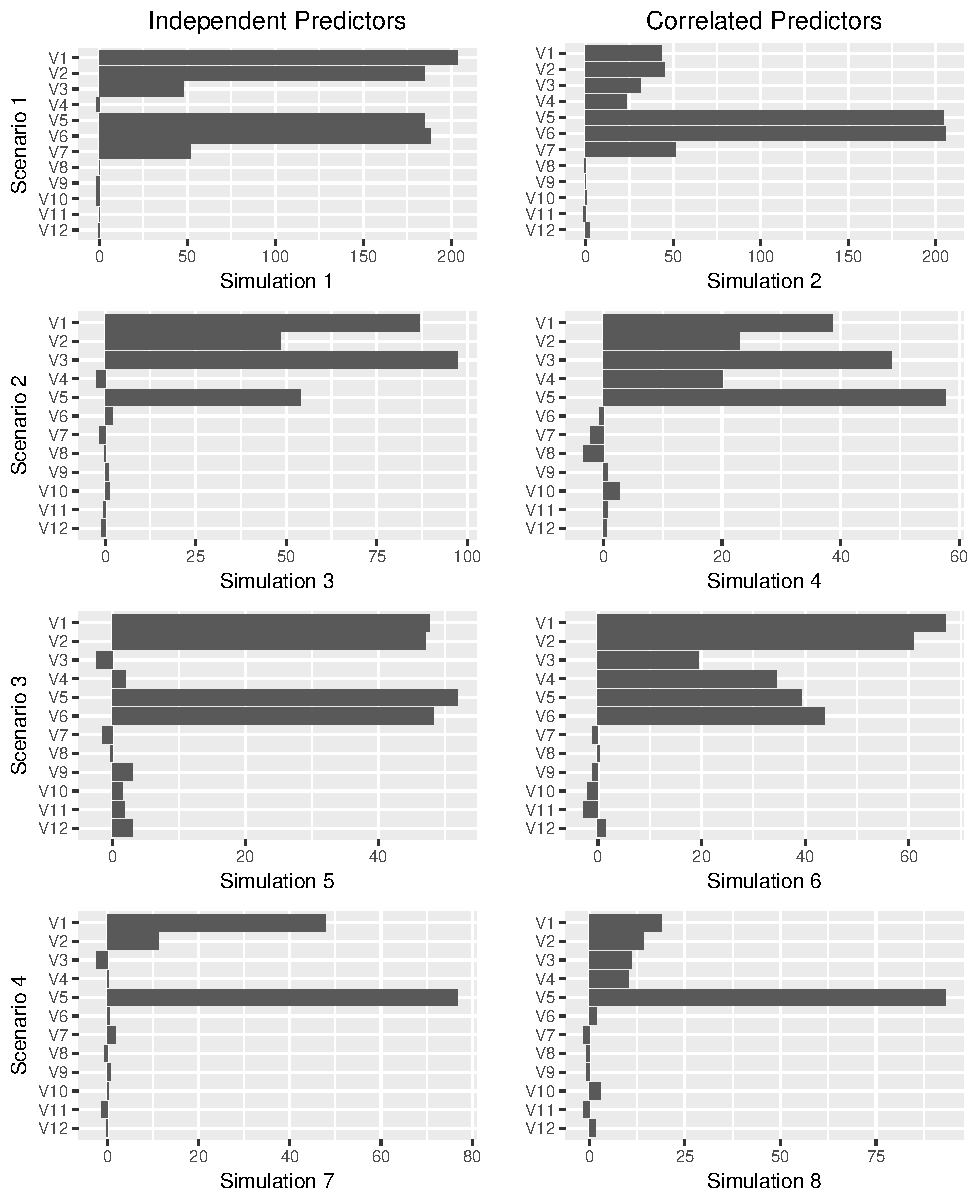
\includegraphics{thesis_files/figure-latex/unnamed-chunk-8-1.pdf}
\caption{\label{fig:unnamed-chunk-8}\label{AVPIwrep}Model-based AVPI
Simulation Results Using Sampling With Replacement}
\end{figure}
\begin{figure}
\centering
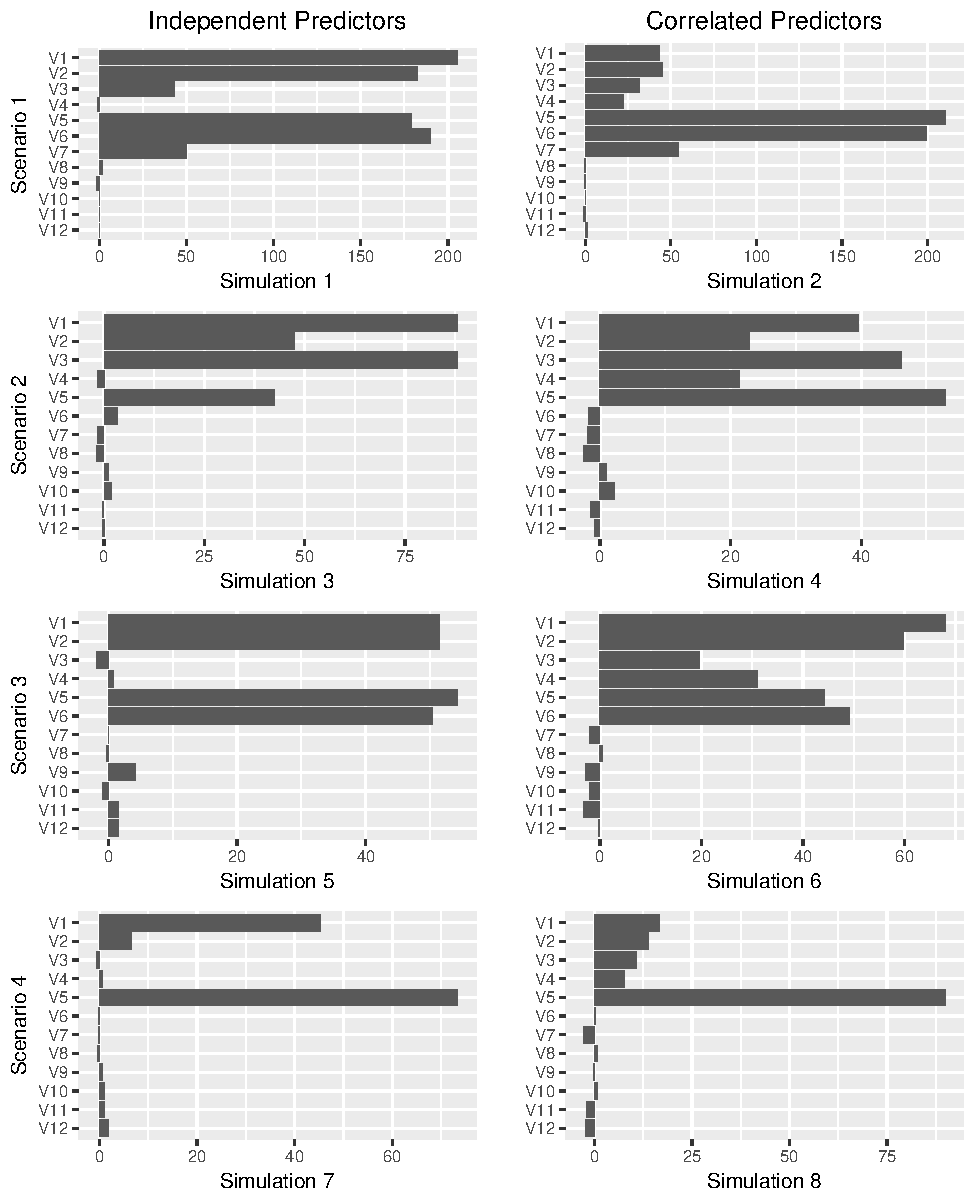
\includegraphics{thesis_files/figure-latex/unnamed-chunk-9-1.pdf}
\caption{\label{fig:unnamed-chunk-9}\label{MDAwrep}MDA Simulation Results
Using Sampling With Replacement}
\end{figure}
For simulation 3 we see that AVPI matches with the MDA variable
importance in matching which variables are informative. However, with
simulation 4, while variable 2 has a higher score than variable 4 with
AVPI and MDA variable importance, both variables have similar scores
with respect to AVPI and MDA variable importance. For simulation 5, the
AVPI scores for variables 1, 2, 5, and 6 were highest although the
uninformative predicotrs had relatively high AVPI scores. For simulation
6, which was the interaction terms with correlated predictors, the AVPI
correctly downweights the importance of variables 3 and 4, while
accounting for the importance of variables 1 and 2. With simulation 7
and 8, which was a highly non-linear response, there was small signal
with respect to variable 2, so both AVPI and MDA importance computed low
scores for variable 2. In particular, variable 2 in simulation 8 for
AVPI has a particularly low score. However, for variables 1 and 5 have
high AVPI scores as expected. \par 
\begin{figure}
\centering
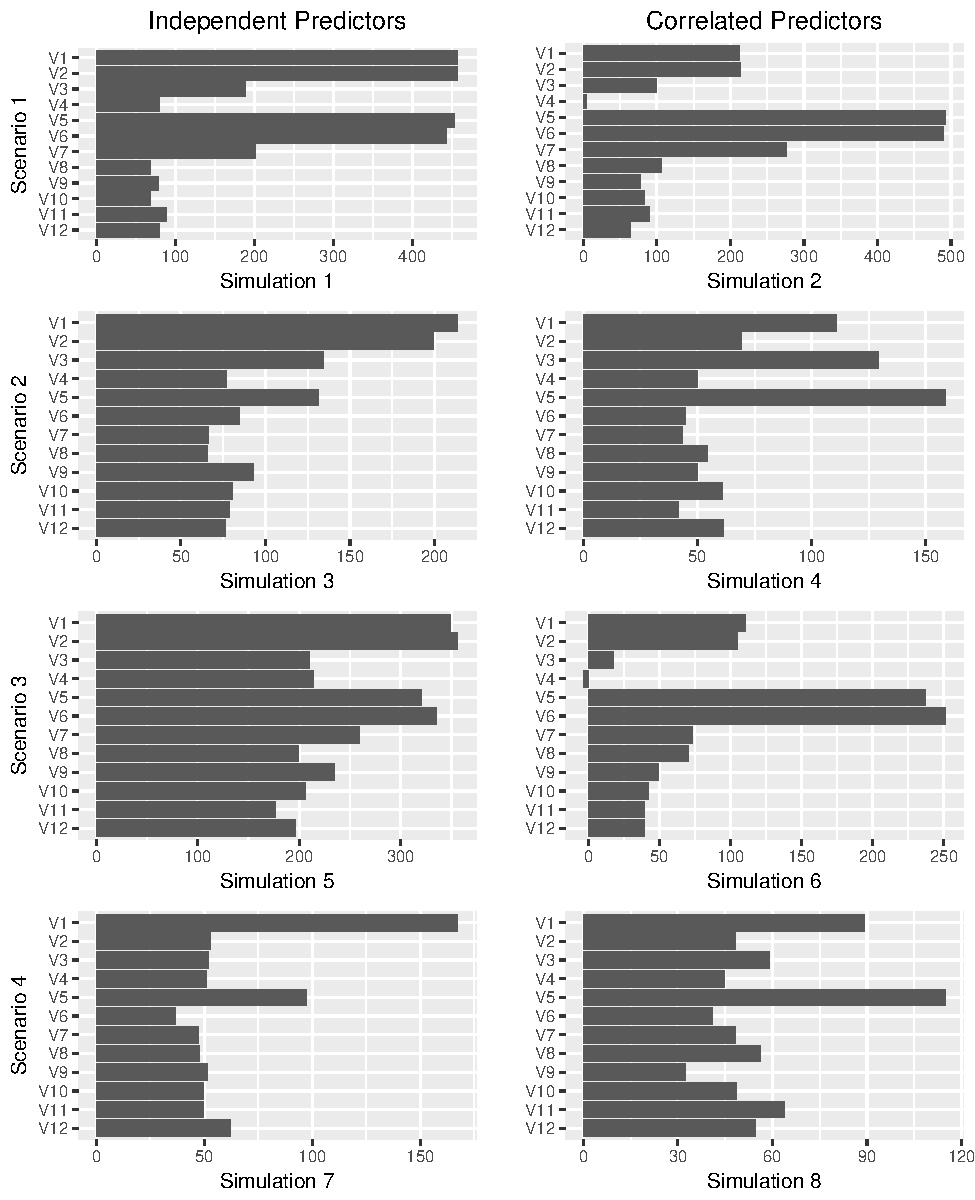
\includegraphics{thesis_files/figure-latex/unnamed-chunk-10-1.pdf}
\caption{\label{fig:unnamed-chunk-10}\label{AVPIworep}Model-based AVPI
Simulation Results Using Sampling Without Replacement}
\end{figure}
\begin{figure}
\centering
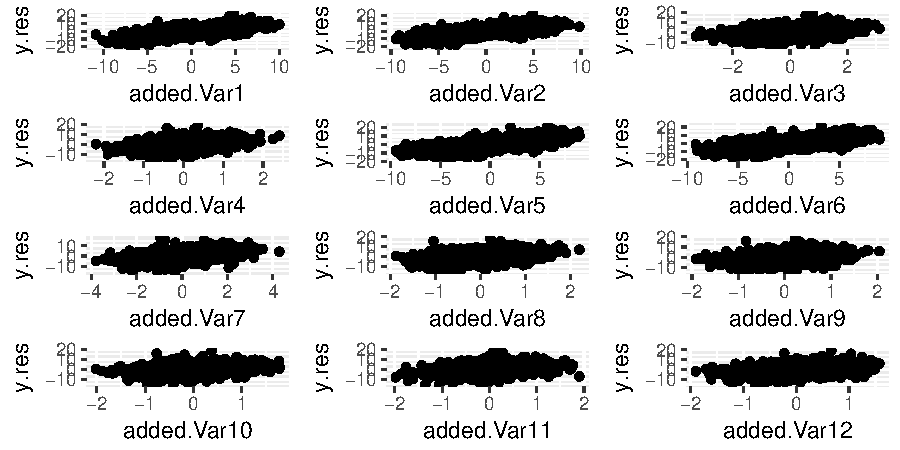
\includegraphics{thesis_files/figure-latex/unnamed-chunk-11-1.pdf}
\caption{\label{fig:unnamed-chunk-11}\label{MDAworep1}MDA Simulation Results
Using Sampling Without Replacement}
\end{figure}
Overall, simulation results indicate that AVPI can determine the
informativeness of predictors with fairly strong signal, although in
general MDA variable importance will offer similar results without the
addition of uninformative variables receiving non-zero scores. In some
situations with correlated predictors, the AVPI appears to find which of
the correlated predictors are informative, so long as the signal in the
informative predictor is relatively strong. This indicates that AVPI may
be most effective as a tool employed alongside MDA variable importance
when there is some correlation structure present in the predictors. In
general, MDA variable importance will be able to evaluate the importance
of independent predictors, and if there is some correlation structure
that leads to unstable MDA variable importance values of the correlated
predictors, then AVPI can be used on just the correlated predictors to
determine which of the correlated predictors are important. \par 
\begin{figure}
\centering
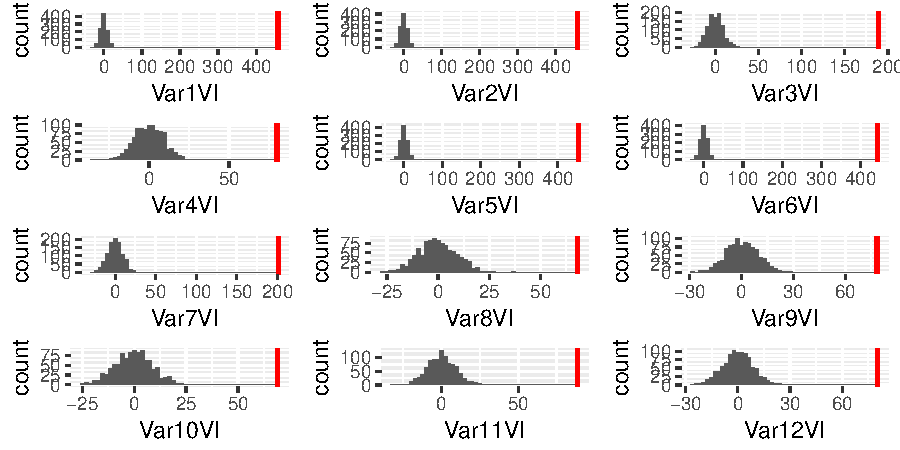
\includegraphics{thesis_files/figure-latex/unnamed-chunk-12-1.pdf}
\caption{\label{fig:unnamed-chunk-12}\label{resAVPI}Residuals-based AVPI
Simulation Results Using Sampling Without Replacement}
\end{figure}
\begin{figure}
\centering
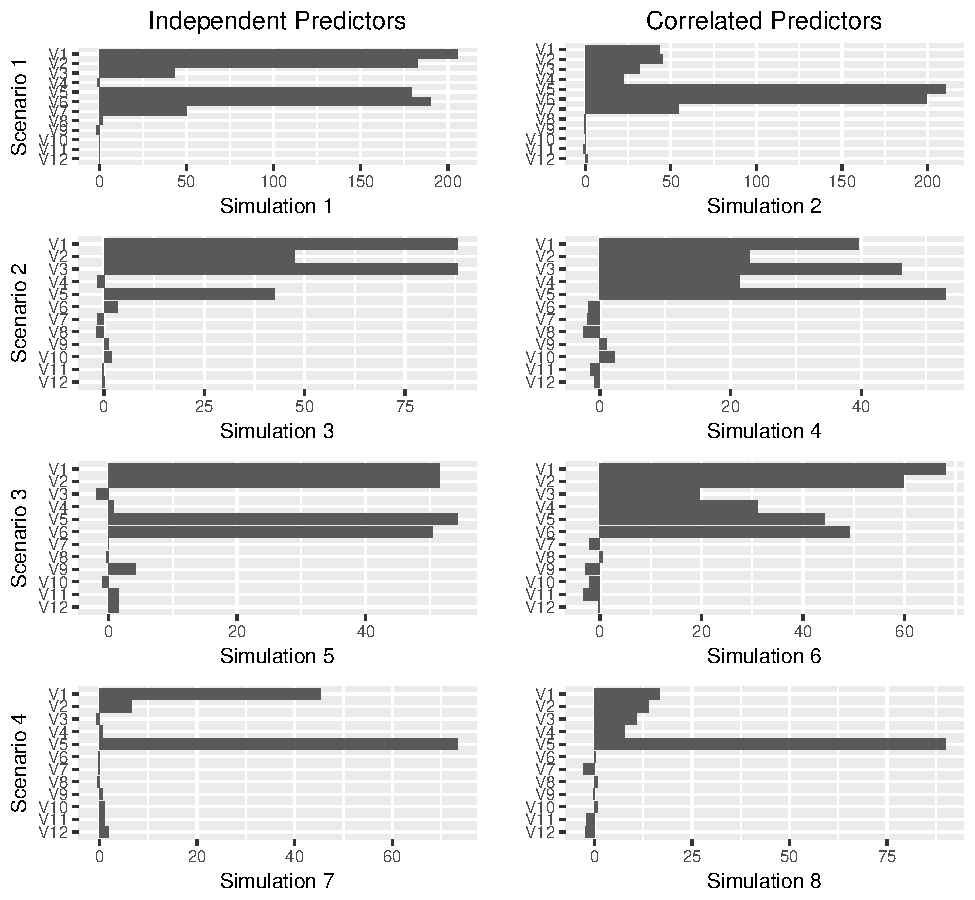
\includegraphics{thesis_files/figure-latex/unnamed-chunk-13-1.pdf}
\caption{\label{fig:unnamed-chunk-13}\label{MDAwrep2}MDA Simulation Results
Using Sampling Without Replacement on same data as in Figure
\ref{resAVPI}}
\end{figure}
One issue with the AVPI method is the relative noisiness of the method.
As observed in the simulation using sampling with replacement,
uninformative variables can be assigned positive AVPI scores. Looking at
results from re-running the simulation using sampling without
replacement, we see that the same sort-of noisiness is also present in
AVPI computed via random forests using sampling without replacement.
Therefore the issue of noisiness for the AVPI method is not simply a
matter of sampling with replacement versus sampling without replacement.
The particular issue with the noisiness of the AVPI method is that it
prevents us from readily employing permutation tests to determine
importance of variables using AVPI as a test statistic in a hypothesis
testing framework. In particular, looking at the tables of AVPI p-values
for both sampling with replacement and sampling without replacement, we
see that both tables are essentially identical, and that under a
hypothesis testing framework, we would be committing type I errors
across all simulations using a significance level of \(\alpha = 0.05\).
Furthermore, looking at the simulated null distribution of AVPI values,
we see that the null distributions are generally quite similar. The
simulated null distribution of AVPI values is generally symmetric with
the lower end of the tails at around an importance score of 25. So any
AVPI score above 30 would likely appear statistically significant using
a permutation test with AVPI as the test statistic. \par
\begin{table}

\caption{\label{tab:unnamed-chunk-14}Added Variable Importance P-values for Sampling with Replacement}
\centering
\resizebox{\linewidth}{!}{\begin{tabular}[t]{lrrrrrrrr}
\toprule
  & Simulation 1 & Simulation 2 & Simulation 3 & Simulation 4 & Simulation 5 & Simulation 6 & Simulation 7 & Simulation 8\\
\midrule
Variable 1 P-Value & 0.001998 & 0.0019980 & 0.001998 & 0.001998 & 0.001998 & 0.0019980 & 0.001998 & 0.001998\\
Variable 2 P-Value & 0.001998 & 0.0019980 & 0.001998 & 0.001998 & 0.001998 & 0.0019980 & 0.001998 & 0.001998\\
Variable 3 P-Value & 0.001998 & 0.0019980 & 0.001998 & 0.001998 & 0.001998 & 0.6573427 & 0.001998 & 0.001998\\
Variable 4 P-Value & 0.001998 & 0.1398601 & 0.001998 & 0.001998 & 0.001998 & 0.0059940 & 0.001998 & 0.001998\\
Variable 5 P-Value & 0.001998 & 0.0019980 & 0.001998 & 0.001998 & 0.001998 & 0.0019980 & 0.001998 & 0.001998\\
\addlinespace
Variable 6 P-Value & 0.001998 & 0.0019980 & 0.001998 & 0.001998 & 0.001998 & 0.0019980 & 0.001998 & 0.001998\\
Variable 7 P-Value & 0.001998 & 0.0019980 & 0.001998 & 0.001998 & 0.001998 & 0.0019980 & 0.001998 & 0.001998\\
Variable 8 P-Value & 0.001998 & 0.0019980 & 0.001998 & 0.001998 & 0.001998 & 0.0019980 & 0.001998 & 0.001998\\
Variable 9 P-Value & 0.001998 & 0.0019980 & 0.001998 & 0.001998 & 0.001998 & 0.0279720 & 0.001998 & 0.001998\\
Variable 10 P-Value & 0.001998 & 0.0019980 & 0.001998 & 0.001998 & 0.001998 & 0.0219780 & 0.001998 & 0.001998\\
\addlinespace
Variable 11 P-Value & 0.001998 & 0.0019980 & 0.001998 & 0.001998 & 0.001998 & 0.0439560 & 0.001998 & 0.001998\\
Variable 12 P-Value & 0.001998 & 0.0019980 & 0.001998 & 0.001998 & 0.001998 & 0.0019980 & 0.001998 & 0.001998\\
\bottomrule
\end{tabular}}
\end{table}
\begin{table}

\caption{\label{tab:unnamed-chunk-15}Added Variable Importance P-values for Sampling without Replacement}
\centering
\resizebox{\linewidth}{!}{\begin{tabular}[t]{lrrrrrrrr}
\toprule
  & Simulation 1 & Simulation 2 & Simulation 3 & Simulation 4 & Simulation 5 & Simulation 6 & Simulation 7 & Simulation 8\\
\midrule
Variable 1 P-Value & 0.001998 & 0.0019980 & 0.001998 & 0.001998 & 0.001998 & 0.0019980 & 0.001998 & 0.001998\\
Variable 2 P-Value & 0.001998 & 0.0019980 & 0.001998 & 0.001998 & 0.001998 & 0.0019980 & 0.001998 & 0.001998\\
Variable 3 P-Value & 0.001998 & 0.0019980 & 0.001998 & 0.001998 & 0.001998 & 0.6573427 & 0.001998 & 0.001998\\
Variable 4 P-Value & 0.001998 & 0.1398601 & 0.001998 & 0.001998 & 0.001998 & 0.0059940 & 0.001998 & 0.001998\\
Variable 5 P-Value & 0.001998 & 0.0019980 & 0.001998 & 0.001998 & 0.001998 & 0.0019980 & 0.001998 & 0.001998\\
\addlinespace
Variable 6 P-Value & 0.001998 & 0.0019980 & 0.001998 & 0.001998 & 0.001998 & 0.0019980 & 0.001998 & 0.001998\\
Variable 7 P-Value & 0.001998 & 0.0019980 & 0.001998 & 0.001998 & 0.001998 & 0.0019980 & 0.001998 & 0.001998\\
Variable 8 P-Value & 0.001998 & 0.0019980 & 0.001998 & 0.001998 & 0.001998 & 0.0019980 & 0.001998 & 0.001998\\
Variable 9 P-Value & 0.001998 & 0.0019980 & 0.001998 & 0.001998 & 0.001998 & 0.0279720 & 0.001998 & 0.001998\\
Variable 10 P-Value & 0.001998 & 0.0019980 & 0.001998 & 0.001998 & 0.001998 & 0.0219780 & 0.001998 & 0.001998\\
\addlinespace
Variable 11 P-Value & 0.001998 & 0.0019980 & 0.001998 & 0.001998 & 0.001998 & 0.0439560 & 0.001998 & 0.001998\\
Variable 12 P-Value & 0.001998 & 0.0019980 & 0.001998 & 0.001998 & 0.001998 & 0.0019980 & 0.001998 & 0.001998\\
\bottomrule
\end{tabular}}
\end{table}
\begin{figure}
\centering
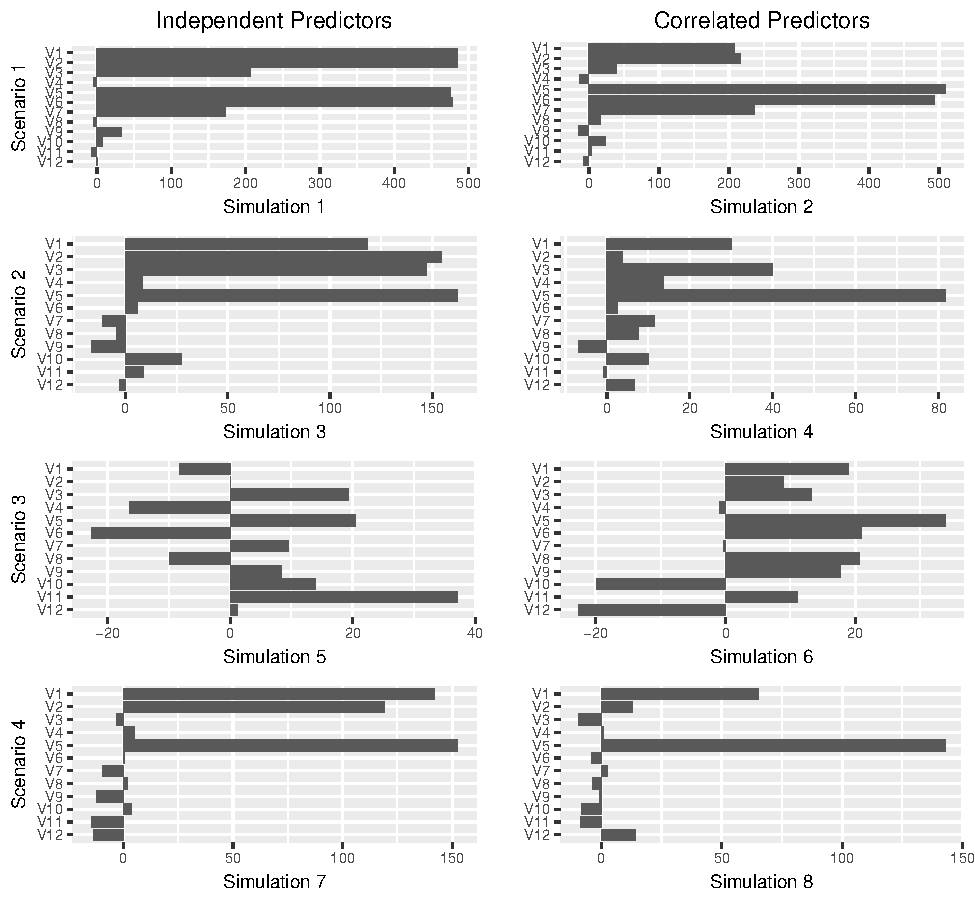
\includegraphics{thesis_files/figure-latex/unnamed-chunk-16-1.pdf}
\caption{\label{fig:unnamed-chunk-16}\label{AVPIdistsiml}Simulated Null
Distributions of AVPI for Each Predictor of Simulation 1 When Sampling
Without Replacement}
\end{figure}
Thus while the AVPI may not be a stable test statistic for use in a
hypothesis testing framework, our simulation results suggest that when
used in conjunction with the MDA variable importance, the AVPI can be a
useful tool for dealing with correlated predictors in a regression
setting. \par

\chapter{Joint Added Variable Plot
Importance}\label{joint-added-variable-plot-importance}

\section{Introduction}\label{introduction-4}

In the previous chapters, we introduced the added variable plot
importance (AVPI) of a predictor in the random forest ensemble. One
direction we can extend our framework of added variable plot importances
is to compute the joint added variable plot importance for a set of
predictors. We would like to capture the joint effect of sets of
predictors on the performance of the random forest ensemble in
predicting the response. One scenario in which we might want to capture
the joint effect of sets of predictors is if out of a set of correlated
predictors, we believe that only a subset of the correlated predictors
are informative to the response. In such a scenario, we would like a
quantitative measure to compare the joint importance of the subset of
correlated informative predictors with the subset of correlated
uninformative predictors. \par

\section{Partial F-Test}\label{partial-f-test}

In the linear regression context, we may be interested in if a subset of
predictors are informative or not towards the linear regression model.
If our covariates are \(\mathbf{X}\), then we would partition the
covariates to \(\mathbf{X}=(\mathbf{X}_1,\mathbf{X}_2)\), where
\(\mathbf{X}_1\) are the first \(p-q\) predictors and \(\mathbf{X}_2\)
are the last \(q\) predictors. Similarly partition the coefficients from
the linear model \(\mathbf{\beta}=(\mathbf{\beta}_1,\mathbf{\beta}_2)\),
where \(\mathbf{\beta}_1\) are the coefficients for the first \(p-q\)
predictors and \(\mathbf{\beta}_2\) are the coefficents for the last
\(q\) predictors. Then we would like to test whether
\(\mathbf{\beta}_2\) should be non-zero for \(\mathbf{X}_2\). We are
testing the hypotheses
\begin{align}
H_0: \mathbf{Y}&=\mathbf{X}_1\mathbf{\beta}_1+\varepsilon \nonumber \\
H_1: \mathbf{Y}&=\mathbf{X}_1\mathbf{\beta}_1+\mathbf{X}_2\mathbf{\beta}_2+\varepsilon. \nonumber
\end{align}
The partial F-test allows us to test the above hypotheses. First fit the
model under the null hypothesis \(H_0\) and find the residual sums of
squares \(RSS_{H_0}\) and degrees of freedom \(df_{H_0}\) of the model.
Next fit the model under the alternative hypothesis \(H_1\) and find
\(RSS_{H_1}\) and \(df_{H_1}\). As Weisberg (2005) notes,
\(df_{H_0}>df_{H_1}\) and \(RSS_{H_0}-RSS_{H_1}>0\). The partial F-test
statistic is
\[F=\frac{(RSS_{H_0}-RSS_{H_1})/(df_{H_0}-df_{H_1})}{RSS_{H_1}/df_{H1}}.\]
If \(F\) is large when compared to the
\(F(df_{H_0}-df_{H_1}, df_{H_1})\) distribution, then there is evidence
against the null hypothesis that the coefficients of
\(\mathbf{\beta}_2\) should be set to zero. In particular, while we
cannot compute a test statistic similar to the F-test statistic for
joint added variable importance, we can take the approach of comparing
models fit with and without \(\mathbf{X}_2\) to determine the importance
of \(\mathbf{X}_2\) in the random forest context. \par

\section{Joint Added Variable Plots}\label{joint-added-variable-plots}

Suppose that out of a particular set of correlated predictors, we
believe that two, \(X_j\) and \(X_k\), are particularly informative to
the response while the other correlated predictors are uninformative.
Denote the set of correlated precictors by
\(H=\{X_{\alpha_1},\ldots,X_{\alpha_m}\}\) of which \(K=\{X_j,X_k\}\) is
a subset. One approach to determining the relative importance of the
variables in \(H\) is to plot added variable plots and compute added
variable plot importances for each variable in \(H\). However, if based
on looking at the full random forest model variable importance, or based
on some other information, we think that the variables in \(K\) are more
important, we could instead train a random forest excluding the
variables in \(K\), a random forest excluding the variables in
\(H\setminus K\), and a random forest excluding the variables in \(H\).
From there we can compute and compare added variable plots and added
variable plot importances for predictors in the set \(K\), the set
\(H\setminus K\), and the set \(H\), respectively, as we would in the
single variable added variable plot scenario. \par

More generally, suppose we have a subset
\(J=\{X_{\alpha_1},\ldots, X_{\alpha_m}\}\subseteq \{X_1,\ldots,X_p\}\),
where \(m< p\), for which we are interested in the joint added variable
effect of the predictors in \(J\). As in the case of the added variable
plot of a single variable, we could grow the full random forest
\(\hat{\theta}_{RF}(Y|X)\) and the reduced model
\(\hat{\theta}_{RF}(Y|X_{-J})\), where \(X_{-J}\) denotes the set of
predictors not in \(J\). The joint added variable plot for the
predictors in \(J\) is then given by
\[(\hat{\theta}_{RF}(Y|X)-\hat{\theta}_{RF}(Y|X_{-J}), Y-\hat{\theta}_{RF}(Y|X_{-J})).\]
The rationale for forming the joint added variable plot of the
predictors in \(J\) is similar to the single variable case, although
care has to be taken in describing what sort-of relationship the joint
added variable plot of \(J\) provides. The joint added variable plot for
\(J\) captures the aggregated informativeness of the predictors in \(J\)
with respect to the response. In particular, if at least one predictor
in \(J\) is informative, then we would expect that the random forest
ensemble \(\hat{\theta}_{RF}(Y|X_{-J})\) would have a decrease in
predictive performance in comparison to the full model. If many
predictors in \(J\) are informative, then we would expect that,
correspondedly there would be a large decrease in predictive performance
in \(\hat{\theta}_{RF}(Y|X_{-J})\). At each node split, as the
predictors in \(J\) are unavailable to be chosen as one of the
\(m_{try}\) variables, there is a greater chance for an uninformative
variable to be chosen as the splitting variable. On the other hand, if
no variable in \(J\) is informative, then we would expect
\(\hat{\theta}_{RF}(Y|X_{-J})\) to have similar predictive performance
to the full model \(\hat{\theta}_{RF}(Y|X)\). Hence for reasons similar
to the single added variable plots, if at least one variable in \(J\) is
an informative predictor of the response, the trend of the joint added
variable plot will be strongly non-zero, while if no predictor in \(J\)
is informative, we would expect the joint added variable plot to be
centered about the origin and have no significant trend. If there are a
mixture of informative and uninformative variables contained in \(J\),
then the joint added variable plot of \(J\) would have a non-zero trend
although the magnitude and direction of the trend would depend on the
composition of the variables in \(J\). \par

Depending on the number of predictors in \(J\) relative to number of
predictors not in \(J\), computing the joint added variable plot for
\(J\) can be quicker than computing the individual added variable plots
of each variable in \(J\). Once the variables in \(J\) are removed,
there are fewer potential splitting variables for the tree growing
algorithm to search through at each split on each node. We would also
recommend when computing the joint added variable plot of \(J\), to also
compute the joint added variable plot of the predictors not in \(J\),
that is to also compute the random forest \(\hat{\theta}_{RF}(Y|X_J)\).
Doing so allows us to compare the predictive value of
\(\hat{\theta}_{RF}(Y|X_{-J})\) and \(\hat{\theta}_{RF}(Y|X_J)\), while
allowing us to also compare the added variable effect of \(J\) versus
the complement of \(J\). \par

{[}Have examples here. One of correlated predictors, another of
uncorrelated predictors{]} \par

\section{Joint Added Variable Plot
Importance}\label{joint-added-variable-plot-importance-1}

As with the single variable case, once we have acquired the joint added
variable plot for \(J\), we would like to have a quantitative measure of
the joint importance of \(J\). As with added variable plot importance,
once we have acquired the joint added variable plot of \(J\),
\[(\hat{\theta}_{RF}(Y|X)-\hat{\theta}_{RF}(Y|X_{-J}), Y-\hat{\theta}_{RF}(Y|X_{-J})),\]
we can try to model the trend in the joint added variable plot utilizing
a bagged forest. Let
\(U_J=\hat{\theta}_{RF}(Y|X)-\hat{\theta}_{RF}(Y|X_{-J})\) and
\(W_J=Y-\hat{\theta}_{RF}(Y|X_{-J})\). To measure, the joint added
variable importance, grow the bagged forest
\(\hat{\theta}_{BF}(W_J|U_j)\) and compute the MDA variable importance
of \(U_J\) in predicting \(W_J\). We call the MDA variable importance of
\(U_J\) the joint added variable importance (JAVPI) of \(J\) and denote
the quantity by \(VI_{JAVP}(X_J)\). Note that the joint added variable
plot importance of \(J\) provides a quantitative measure of the relative
importance of \(U_J\) in predicting the trend in the added variable
plot. As mentioned previously, the trend in the added variable plot of
\(J\) should reflect the aggregated informativeness of the variables in
\(J\) with respect to the response, so the JAVPI of \(J\) indicates the
relative aggregated importance of the variables in \(J\) as predictors
of the response. In particular, higher values of JAVPI for \(J\) should
indicate that the variables contained in \(J\) are more informative than
lower values of JAVPI for \(J\). That is, the value of JAVPI measures
the importance of all the predictors in \(J\) to the response \(Y\) via
the loss in predictive performance in the ensemble when we remove the
predictors in \(J\) as potential splitting variables in the forest
growing process. As in the previous section, we also recommend that
\(VI_{JAVP}(X_{-J})\), the JAVPI of those predictors not in \(J\) be
concurrently computed to provide a comparison of joint importance
between sets of predictors. \par
\begin{algorithm}
    \caption{Joint Added Variable Plot Importance (JAVPI)} \label{added variable importance}
      \begin{algorithmic}[1]
          \State Grow the random forest ensemble $\hat{\theta}_{RF}(Y|X)$ predicting $Y$ using the full set of predictors.
          \State Grow the random forest ensemble $\hat{\theta}_{RF}(Y|X_{-J})$ predicting $Y$ using the full set of predictors minus the predictors in $J$.
          \State Compute $U_J=\hat{\theta}_{RF}(Y|X)-\hat{\theta}_{RF}(Y|X_{-J})$ and $W_J=Y-\hat{\theta}_{RF}(Y|X_{-J})).$
          \State Grow the bagged forest ensemble $\hat{\theta}_{BF}(W_J|U_J)$ predicting $W_J$ using $U_J$. 
          \State Compute the added variable plot importance of $X_J$ to be the MDA variable importance of $U_J$: $VI_{JAVP}(X_J)=VI_{MDA}(U_J)$.
          
      \end{algorithmic}
  \end{algorithm}
\section{Permutation Tests Using Joint Added Variable Plot
Importance}\label{permutation-tests-using-joint-added-variable-plot-importance}

Once we have computed \(VI_{JAVP}(X_J)\), we can again take a simulation
approach to generating a sampling distribution for \(VI_{JAVP}(X_J)\).
The process is essentially analogous to computing sampling distributions
of single added variable plots. To compute \(VI_{JAVP}(X_J)\), we
require the joint added variable plot \((U_J,W_J)\), where
\(U_J=\hat{\theta}_{RF}(Y|X)-\hat{\theta}_{RF}(Y|X_{-J})\) and
\(W_J=Y-\hat{\theta}_{RF}(Y|X_{-J})\). Permute \(U_J\) to obtain
\(U_J^*\) and grow the bagged forest \(\hat{\theta}_{BF}(W_J|U_J^*)\)
using the permuted \(U_J^*\) as the predictor. We then use the resulting
ensemble to compute \(VI_{MDA}(U_J^*)=VI_{JAVP}^*(X_J)\) as the permuted
JAVPI of \(J\). Once we have ran enough iterations of permutations of
\(U_J^*\) and computation \(VI_{JAVP}^*(X_J)\), we can compute a
two-sided p-value using \(VI_{JAVP}(X_J)\) as our test statistic. \par

If we have a collection \(J_1,\ldots, J_q\) of subsets of the
predictors, we could simulate sampling distributions of
\(VI_{JAVP}(X_{J_i})\) for each \(i=1,\ldots,q\) and compute two-sided
p-values for each subset \(J_i\). We could then enter into a hypothesis
testing framework. We do offer some words of caution here with respect
to using joint added variable plot importances in a hypothesis test
framework with multiple subsets. In particular, due to sensitivity of
permutation tests using JAVPI to type-I errors and due to possible
overlap of predictors in the \(J_i\), we would recommend most certainly
using a multiple comparisons procedure such as the Bonferonni
correction. Furthermore, we would like to emphasize the use of JAVPI and
AVPI as variable selection tools and diagnostic tools for random
forests, rather than tools purely of inferential statistics and
hypothesis testing. \par

With the JAVPI, in particular, our intention in introducing the JAVPI
variable importance measure was to offer a method that utilizes the
random forest mechanism to measure the importance of a subset \(J\) of
predictors while taking into account the effect of the predictors not in
\(J\). However, as we have noted above, if the subset \(J\) of
predictors consists of a mixture of informative and uninformative
predictors, then a finer analysis of the variables in \(J\) may be
required if the JAVPI of \(J\) is high. Concluding that each variable in
\(J\) is informative based on a high JAVPI value or low p-value from
simulation would be erronuous if \(J\) is a mixture of informative and
uninformative. We would also like to emphasize that it is important to
check the fit and residual sum of squares of the random forest model if
using the JAVPI or AVPI to see if conclusions drawn from JAVPI or AVPI
are valid. Furthermore, we would like to remind the reader that
inference based on residuals as we are describing with JAVPI and AVPI
can be sensitive to outliers and extreme points such that statistically
significant results from JAVPI or AVPI should be examined with some
scrutiny. \par

\section{Simulation and Results of Joint Added Variable Plot
Importance}\label{simulation-and-results-of-joint-added-variable-plot-importance}

\subsection{Simulation Design}\label{simulation-design-1}

For our simulation of JAVPI, we used our simulation set-up from chapter
4 with some changes. That is we ran the 8 simulations from chapter 4
where we have independent and correlated predictors for each scenario.
Rather than test both sampling with replacement and sampling without
replacement for JAVPI, we chose to run our simulation on JAVPI with just
sampling without replacement. In addition, we ran two sets of
simulations for JAVPI to illustrate different features of the method.
The first simulation was a simulation where we partitioned out all of
the informative predictors to the response, leaving no signal in the
remaining data. For the second simulation, we partitioned out our
predictors such that both partitions of the set of predictors contained
informative predictors. In the tables below we show the partitions of
our simulated data sets for both the first round and second round of
simulations. All other settings for the simulations are the same as
those for chapter 4: we drew 2000 samples and grew 1000 tree ensembles
for both stages of JAVPI. \par 
\begin{table}

\caption{\label{tab:unnamed-chunk-20}Partitions for Simulation Runs 1 and 2, respectively}
\centering
\resizebox{\linewidth}{!}{\begin{tabular}[t]{lll}
\toprule
  & Partition of Predictors & Partition of Predictors\\
\midrule
Scenario 1 & V1, V2, V3, V5, V6, V7 & V1, V2, V3\\
Scenario 2 & V1, V2, V3, V5 & V1, V2\\
Scenario 3 & V1, V2,V5, V6 & V1, V2\\
Scenario 4 & V1, V2, V5 & V1, V2\\
\bottomrule
\end{tabular}}
\end{table}
\section{Simulation Results}\label{simulation-results-1}

Below are simulation results of JAVPI for the first simulation run. We
find that, in general, JAVPI is relatively stable at distinguishing
between the set of predictors containing all the signal and the set of
predictors that are noise. In particular, in all cases the JAVPI values
are much higher for the set of informative predictors than for the set
of uninformative predictors, which is what we expected. We do note that
in simulations 1, 2, and 6, the JAVPI value for the uninformative
predictors is quite high. Some possible reasons for this are monte carlo
variability and relatively weak signal in the predictors allowing for
some masking between variables. \par 
\begin{figure}
\centering
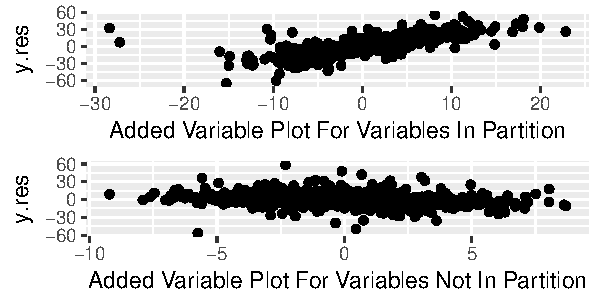
\includegraphics{thesis_files/figure-latex/unnamed-chunk-21-1.pdf}
\caption{\label{fig:unnamed-chunk-21}\label{JAVPIonesig}JAVPI Simulation
Results When All the Signal is Contained in the Partition}
\end{figure}
We examine the joint added variable plots for simulations 1, then
simulation 2. \par 
\begin{figure}
\centering
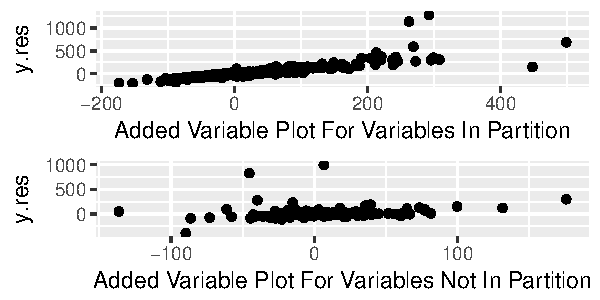
\includegraphics{thesis_files/figure-latex/unnamed-chunk-22-1.pdf}
\caption{\label{fig:unnamed-chunk-22}\label{siml1to5plots}JAVP for
Simulations 1, 2, and 5, Respectively, for First Simulation Run}
\end{figure}
We see that there is a weak negative trend among the uninformative
variables. This structure is somewhat hard to explain, although it is
most likely due to noise or masking among variables. We do note that the
informative predictors have a strongly positive trend in contrast to the
uninformative predictors. This is in contrast to the joint added
variable plots for simulations 5 below. \par 

For simulation 5, the uninformative variables had no trend while the
informative variables had a strong positive trend. This at least
indicates that the JAVPI score captures the relative structure present
in the joint added variable plot. For lower values of JAVPI, we do not
expect there to be much structure in the joint added variable plot,
indicating uninformativeness of those variables. Higher values of JAVPI
indicate that there is structure in data. In the case of higher JAVPI
scores, combining the JAVPI score with the joint added variable plot
should allow us to figure out where the signal is present. For example,
with simulations 1 and 2, the trend of the joint added variable plot for
the informative variables is much stronger than the trend for the
uninformative variables. Furthermore, the JAVPI score for the
informative variables is much higher than the JAVPI scores for the
uninformative variables. Some further testing, such as examining the MDA
variable importance for the full set of predictors may then allow us to
conclude that the set of uninformative variables are truly
uninformative. If the set of uninformative variables is not too large,
we could also try computing the JAVPI for each predictor in the set of
uninformative variables individually. If there is some signal in those
predictors, then we would expect there to be some non-zero trend in the
resulting joint added variable plot, otherwise, there would be no trend
in the joint added variable plot. \par 
\begin{figure}
\centering
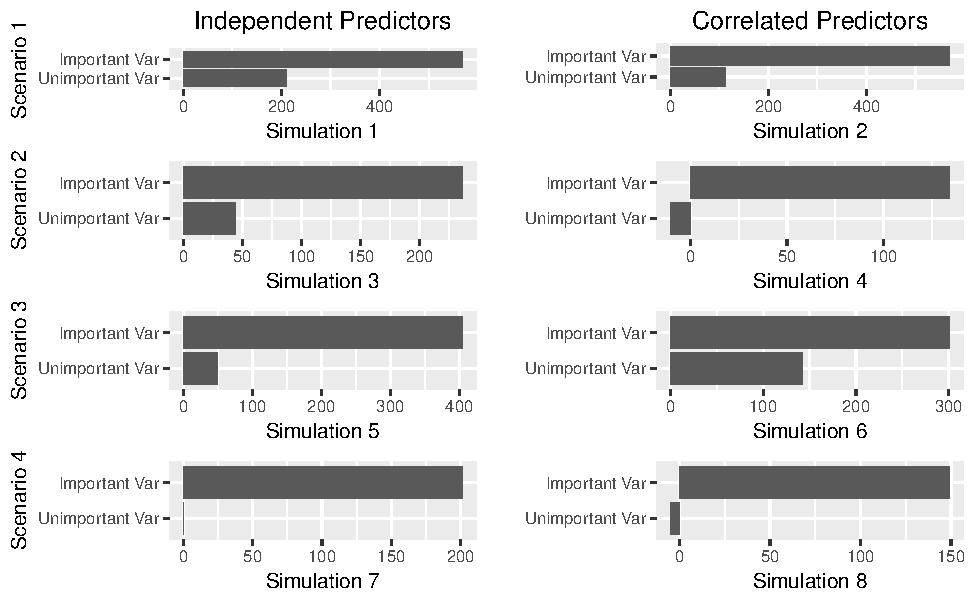
\includegraphics{thesis_files/figure-latex/unnamed-chunk-23-1.pdf}
\caption{\label{fig:unnamed-chunk-23}\label{MDAforJAVPI} MDA Simulation
Results for JAVPI Simulated Datasets}
\end{figure}
For the second simulation run, where there was signal in both partitions
of the predictors, we find that, in general, the JAVPI scores for both
partitions in each simulation is high, as we expected. When we include
signal in both partitions, the JAVPI will generally pick up on the
signal, and we can examine the joint added variable plots for visual
confirmation of what is going on. In particular, we display the joint
added variable plot for simulation 1. \par 
\begin{figure}
\centering
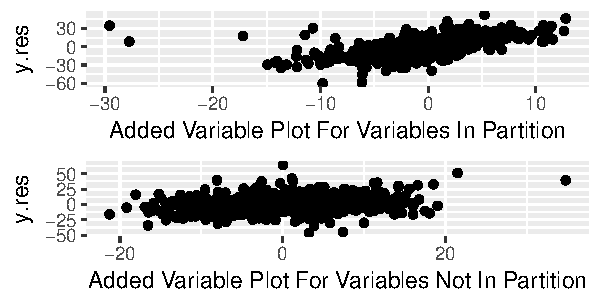
\includegraphics{thesis_files/figure-latex/unnamed-chunk-24-1.pdf}
\caption{\label{fig:unnamed-chunk-24}\label{JAVPItwosig}JAVPI Simulation
Results When Signal is Contained in Both Partitions of the Predictors}
\end{figure}
\begin{figure}
\centering
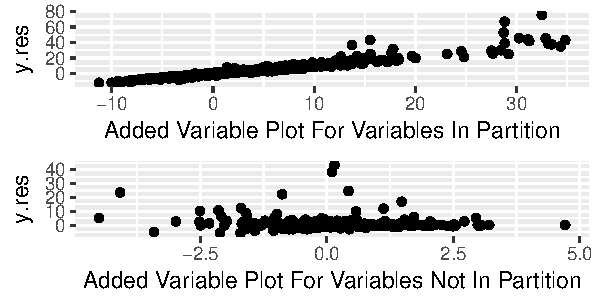
\includegraphics{thesis_files/figure-latex/unnamed-chunk-25-1.pdf}
\caption{\label{fig:unnamed-chunk-25}\label{siml1and5plots}JAVP for
Simulations 1 and 5, Respectively, for Second Simulation Run}
\end{figure}
For simulation 1, we found the JAVPI scores for both partitions is quite
similar (around 512 versus 492), which makes sense given that we split
the informative predictors evenly between both predictors. The joint
added variable plot for simulation 1 is a strong positive trend as
expected given the size of the JAVPI scores. \par 

On the other hand, examining the table of JAVPI values for the second
simulation run, it seems that in simulation 5, the second partition had
a much lower JAVPI score than the first partition. Examining the joint
added variable plots for simulation 5 immediately above, we see that
while the joint added variable plot for the first partition is strongly
positive, we can only describe the trend in the joint added variable
plot for the second partition as being weakly positive. The JAVPI score
for the second partition is high enough to suggest that there is signal
in the second partition, but is much lower than the JAVPI score for the
first partition. This seems very likely to be due to monte carlo
variability. Choosing a different seed and re-running simulation 5
results in a appropriately high JAVPI value for the second partition,
which is what we had expected. \par 

We conclude this chapter by noting that throughout our simulations for
JAVPI, the conclusions we reached with respect to independent versus
correlated predictors were quite similar. Since with JAVPI, we are
interested in the aggregated effect of a set of predictors, this means
that we are really testing whether or not the subset of predictors
contains a discernable signal. The particular usefulness of JAVPI is not
necessarily detecting where there is a signal, but detecting where there
is not a signal. If a subset of predictors produce a low JAVPI score,
then it is quite possible that there is very little to no signal in that
subset. Hence in this manner, we could in theory test each correlated
variable in a data set to try to figure out if any correlated predictors
are informative to the response. Of course, such a method can be
computationally intractible and impractical for data sets with many
predictors, so computing the JAVPI score of different combinations of
subsets could be more efficient than testing each predictor one by one.
Furthermore, the JAVPI score is more computationally efficient to
compute than the AVPI score since for each JAVPI score we train 5 forest
ensembles, while for AVPI, if \(p\) is the number of predictors in the
data set, then to compute the AVPI scores of a data set we would have to
train \(2p+1\) many forest ensembles. This suggests that for
applications to permutation tests when the AVPI and JAVPI scores are not
too noisy, the JAVPI score would be more efficient to compute a
permutation test for. We do note that JAVPI is sensitive to the strength
of the signal in the response. If the signal is weak, then the AVPI and
JAVPI methods will be sensitive to noise, but if the signal in the
response is strong, the AVPI and JAVPI methods will be less sensitive to
noise in the data. \par 

\chapter*{Conclusion}\label{conclusion}
\addcontentsline{toc}{chapter}{Conclusion}

\appendix

\chapter{The First Appendix}\label{the-first-appendix}

\backmatter

\chapter*{References}\label{references}
\addcontentsline{toc}{chapter}{References}

\markboth{References}{References}

\noindent

\setlength{\parindent}{-0.20in} \setlength{\leftskip}{0.20in}
\setlength{\parskip}{8pt}

\hypertarget{refs}{}
\hypertarget{ref-biau2015a}{}
Biau, G., \& Scornet, E. (2016). A random forest guided tour. \emph{E.
TEST}, \emph{25}(2), 197--227.

\hypertarget{ref-breiman1984}{}
Breiman, L., Friedman, J. H., Olshen, R. A., \& Stone, C. J. (1984).
\emph{Classification and regression trees}. New York: Chapman; Hall.

\hypertarget{ref-chen2003}{}
Chen, S. X., \& Hall, P. (2003). EFFECTS of bagging and bias correction
on estimators defined by estimating equations. \emph{Statistica Sinica},
\emph{13}(1), 97--109.

\hypertarget{ref-cook1982}{}
Cook, D. R., \& Weisberg, S. (1982). \emph{Residuals and influence in
regression}. London: Chapman; Hall.

\hypertarget{ref-efron2014}{}
Efron, B. (2014). Estimation and accuracy after model selection.
\emph{Journal of the American Statistical Association}, \emph{109}(507),
991--1007. \url{http://doi.org/doi.org/10.1080/01621459.2013.823775}

\hypertarget{ref-hall1999}{}
Friedman, J., \& Hall, P. (1999). On bagging and nonlinear estimation,
\emph{137}.

\hypertarget{ref-esl2009}{}
Hastie, T., Tibshirani, R., \& Friedman, J. (2009). \emph{The elements
of statistical learning: Data mining, inference and prediction} (2nd
ed.). Springer.

\hypertarget{ref-hothorn2006}{}
Hothorn, T., Hornik, K., \& Zeileis, A. (2006). Unbiased recursive
partitioning: A conditional inference framework. \emph{Journal of
Computational and Graphical Statistics}, \emph{15}(3), 651--674.
\url{http://doi.org/10.1198/106186006X133933}

\hypertarget{ref-ishwaran2007}{}
Ishwaran, H. (2007). Variable importance in binary regression trees and
forests. \emph{Electron J Stat}, 519--537.

\hypertarget{ref-ishwaran2015}{}
Ishwaran, H. (2015). The effect of splitting on random forests.
\emph{Mach. Learn.}, \emph{99}(1), 75--118.
\url{http://doi.org/10.1007/s10994-014-5451-2}

\hypertarget{ref-louppe2014}{}
Louppe, G. (2014). \emph{Understanding random forests from theory to
practice} (PhD dissertation). University of Liège.

\hypertarget{ref-mentch2016b}{}
Mentch, L., \& Hooker, G. (2016a). Formal hypothesis tests for additive
structure in random forests. Retrieved from
\url{http://arxiv.org/abs/1406.1845}

\hypertarget{ref-mentch2016a}{}
Mentch, L., \& Hooker, G. (2016b). Quantifying uncertainty in random
forests via confidence intervals and hypothesis tests. \emph{Journal of
Machine Learning Research}, \emph{17}(26), 1--41. Retrieved from
\url{http://jmlr.org/papers/v17/14-168.html}

\hypertarget{ref-owens2017}{}
Owens, A. (2017). \emph{INFFOREST variable importance for random
forests} (Undergraduate Thesis). Reed College.

\hypertarget{ref-rendahl2008}{}
Rendahl, A. K. (2008). \emph{Graphical methods of determining predictor
importance and effect} (PhD dissertation). University of Minnesota.

\hypertarget{ref-sheather2009}{}
Sheather, S. (2009). \emph{A modern approach to regression with r}. New
York: Springer-Verlag.

\hypertarget{ref-strobl2008}{}
Strobl, C., Boulesteix, A.-L., Kneib, T., Augustin, T., \& Zeileis, A.
(2008). Conditional variable importance for random forests. \emph{BMC
Bioinformatics}, \emph{9}(1), 307.
\url{http://doi.org/10.1186/1471-2105-9-307}

\hypertarget{ref-strobl2007}{}
Strobl, C., Boulesteix, A.-L., Zeileis, A., \& Hothorn, T. (2007). Bias
in random forest variable importance measures: Illustrations, sources
and a solution. \emph{BMC Bioinformatics}, \emph{8}(1), 25.
\url{http://doi.org/10.1186/1471-2105-8-25}

\hypertarget{ref-wager2017}{}
Wager, S., \& Athey, S. (2017). Estimation and inference of
heterogeneous treatment effects using random forests. \emph{Journal of
the American Statistical Association}, \emph{0}(ja), 0--0.
\url{http://doi.org/10.1080/01621459.2017.1319839}

\hypertarget{ref-weisberg2005}{}
Weisberg, S. (2005). \emph{Applied linear regression}. New York: John
Wiley \& Sons.


% Index?

\end{document}
